\documentclass{article}
\usepackage[T1]{fontenc}
\usepackage{helvet}
\renewcommand{\familydefault}{\sfdefault}
\usepackage{listings}
\usepackage[utf8]{inputenc}
\usepackage[english]{babel}
\usepackage{booktabs} % Per linee orizzontali professionali nelle tabelle
\usepackage{longtable} % Per tabelle che possono estendersi su più pagine
\usepackage{xcolor}
\usepackage{setspace}
\usepackage{subcaption}

\onehalfspacing % Per interlinea 1.5
\setlength{\parskip}{0.5em}

% Set page size and margins
\usepackage[letterpaper,top=2cm,bottom=2cm,left=3cm,right=3cm,marginparwidth=1.75cm]{geometry}

\usepackage{xstring}
% Useful packages
\usepackage{amsmath}
\usepackage{amssymb}
\usepackage{graphicx}
% Stile didascalie immagini e label
\usepackage[labelfont=sf,textfont=it,font=small]{caption}

\usepackage{authblk}
\usepackage[colorlinks=true, allcolors=blue]{hyperref}
%\usepackage{orcidlink} % per il logo ORCID - commented out for compilation
\newcommand{\orcidlink}[1]{} % Define empty command to avoid errors

\title{Multiscale Feature Extraction with Wavelet Scattering Transform for Remote Sensing Vegetation Classification via Machine Learning}


\usepackage{titlesec}
\titleformat{\section}
  {\normalfont\Large\bfseries\scshape}{\thesection}{1em}{}
\titleformat{name=\section,numberless}
  {\normalfont\Large\bfseries\scshape}{}{0em}{}
\titleformat{\subsection}
  {\normalfont\large\bfseries\scshape}{\thesubsection}{1em}{}
\titleformat{\subsubsection}
  {\normalfont\normalsize\bfseries\scshape}{\thesubsubsection}{1em}{}



\author[1,*]{Mattia Bruscia\,\orcidlink{0000-0003-0910-6445}}
\author[1]{William Nardin\,\orcidlink{0000-0002-5490-879X}}
\author[1]{Xiaoxu Guo}
\author[1]{Limin Sun}
\author[2]{Giulia Franchi}

\affil[1]{University of Maryland Center for Environmental Science (UMCES), Horn Point Laboratory, Cambridge, MD, USA}
\affil[2]{Department of Computer Science, Salisbury University, Salisbury, MD, USA}

\affil[ ]{\textit{Corresponding author}: mbruscia@umces.edu}

\date{} % Rimuove la data dalla pagina iniziale

\begin{document}
\maketitle

\begin{center}
\textbf{\textsc{Abstract}}
\end{center}

This study evaluates the Wavelet Scattering Transform (WST) as a feature extraction technique for Random Forest-based land cover classification under challenging conditions including limited datasets and noisy imagery. The research was conducted at three coastal sites in the Chesapeake Bay region (Maryland, USA): Poplar Island (ecological restoration site), Assateague Island (natural barrier island), and Sunset Island (urban coastal environment). These sites represent diverse ecological conditions with varying degrees of anthropogenic impact.

The experimental framework comprised 1,512 classification experiments spanning six noise types (Gaussian, Poisson, Salt-and-Pepper, Speckle, Uniform, and clean baseline), three dataset sizes (5--40 images per class), and three feature extraction methods: advanced statistical descriptors, WST, and a hybrid approach combining both.

Key findings demonstrate that the Hybrid method achieves statistically significant improvements over the statistical baseline. The Hybrid approach exhibits superior noise robustness, degrading approximately slower than Advanced Statistics under increasing noise intensity. Under extreme data scarcity (5 images per class), all methods retain over 94\% of baseline performance, indicating strong data efficiency.
However, WST alone does not significantly outperform traditional statistical features, and its computational overhead (approximately 10$\times$ slower than statistical feature extraction) is not consistently justified under low-noise conditions. These results provide practical guidance for Unmanned Aerial Vehicle (UAV)-based ecological monitoring: Hybrid features are recommended for high-noise scenarios with GPU acceleration available, while simpler statistical approaches suffice for clean imagery or resource-constrained deployments.


\textbf{\textsc{Keywords}} 
Features Classification, Wavelet Scattering Transform, Vegetation boundaries detection, Ecological Restoration, Wetland Nature-Based Solution, Drones, Unmanned Aerial Vehicles Imagery


\section{Introduction}

% ============================================================================
% 1. CONTESTO GENERALE - Broad Context
% ============================================================================

Coastal wetlands—including salt marshes, mangroves, and estuaries—are among the most productive and biodiverse ecosystems on Earth. These environments provide critical ecosystem services that directly sustain human well-being, including carbon sequestration and storage (blue carbon), filtration of pollutants and excess nutrients, and natural protection against storm surges and coastal erosion \cite{zedler2005wetland, barbier2011value, Mitsch2013}. Beyond their ecological significance, coastal wetlands contribute substantially to global fisheries, support endemic and threatened species, and generate economic benefits through tourism and resource provisioning for millions of people worldwide.
Despite their recognized importance, coastal wetlands face unprecedented threats from both anthropogenic pressures and natural stressors. Urbanization, agricultural expansion, industrial pollution, and land-use conversion have resulted in widespread habitat fragmentation and biodiversity loss. These challenges are compounded by climate change, which manifests through rising sea levels, altered temperature regimes, ocean acidification, and increased frequency of extreme weather events \cite{worm2006impacts}. Eutrophication—driven by nutrient runoff from agriculture and industry—further destabilizes these ecosystems by promoting harmful algal blooms, depleting oxygen levels, and threatening aquatic life. Salt marshes, in particular, are vulnerable to accelerated erosion and altered sedimentation dynamics caused by hurricanes, storm surges, and chronic sea level rise. Recent studies have also shown that marsh sediments accumulate microplastics in proportion to surrounding urbanization, serving as indicators of anthropogenic impact on coastal environments \cite{lloret2020microplastics}.

% ============================================================================
% 2. CONTESTO SPECIFICO - Remote Sensing and Monitoring
% ============================================================================

Given these escalating threats, the development of effective monitoring systems for coastal wetland ecosystems has become a critical priority. Traditional field-based methods—such as manual vegetation surveys and in situ measurements of biomass—although accurate, are labor-intensive, time-consuming, and impractical for large-scale or inaccessible areas \cite{Xue2017Significant}. Remote sensing technologies, including satellite imagery and Unmanned Aerial Vehicles (UAVs), have emerged as powerful alternatives, enabling efficient, cost-effective, and spatially comprehensive data collection over complex landscapes \cite{Zhang2016Remote}. UAVs, in particular, offer distinct advantages over satellite platforms: ultra-high spatial resolution (sub-centimeter pixel sizes), flexible deployment, multisensor integration (RGB, multispectral, thermal, LiDAR), and operational feasibility under varying weather and illumination conditions. These capabilities have positioned UAVs as essential tools for wetland vegetation mapping \cite{Ma, Correll2019}, invasive species detection, biomass estimation, and ecological restoration monitoring \cite{nardin2020ndvi, wan2014spartina, doughty2019mapping, adade2021uav}.
Long-term monitoring programs in the Chesapeake Bay region exemplify the operational application of UAV-based remote sensing across diverse coastal environments. Poplar Island, reconstructed using dredged sediment to restore tidal marsh habitats, faces ongoing challenges related to erosion, sediment accretion, and vegetation dynamics in a highly engineered ecosystem. Assateague Island, a barrier island managed primarily by the National Park Service, provides a comparative reference representing more natural coastal dynamics with extensive dune systems, maritime forests, and salt marshes shaped by natural processes and selective shoreline stabilization interventions. Sunset Island, located in the Isle of Wight Bay adjacent to Ocean City, represents a managed coastal environment where `living shoreline' restoration projects integrate ecological restoration within heavily urbanized waterfronts, balancing erosion control with habitat enhancement. Across these sites, marsh platform morphology is influenced by complex interactions among vegetation distribution, tidal creek networks, and sediment transport processes. Predictive models and empirical studies have documented significant habitat losses attributable to sea level rise and coastal erosion, underscoring the urgency of developing scalable, automated, and robust monitoring methodologies capable of operating across heterogeneous coastal settings \cite{VALIELA20181148}.

% ============================================================================
% 3. LACUNA DI CONOSCENZA - Knowledge Gap
% ============================================================================

While remote sensing provides unprecedented opportunities for large-scale environmental monitoring, UAV-acquired imagery is inherently susceptible to multiple sources of degradation that limit classification accuracy and model generalizability. Sensor imperfections, atmospheric scattering, variable illumination, motion blur, and environmental factors (e.g., wind-induced vegetation movement, water reflections, shadows) introduce diverse forms of noise into acquired data. These noise sources are particularly problematic in real-world operational scenarios where image quality cannot be controlled. Furthermore, ecological restoration sites—such as newly established marsh platforms—often lack extensive labeled datasets, presenting a fundamental challenge for supervised machine learning approaches that require large training corpora to achieve robust performance.
Traditional feature extraction methods for image classification—such as handcrafted statistical descriptors (mean, variance, skewness, kurtosis, texture features)—provide interpretable and computationally efficient representations but often lack robustness to noise and may not capture complex spatial patterns essential for discriminating between visually similar land cover classes (e.g., different vegetation types, vegetated vs. unvegetated marsh areas). Convolutional Neural Networks (CNNs), while highly effective in clean, large-scale datasets, exhibit reduced performance under noisy conditions and require substantial labeled data for training—a requirement frequently unmet in ecological monitoring contexts. Moreover, CNNs function as black-box models, limiting interpretability and hindering scientific understanding of which image features contribute to classification decisions.

% ============================================================================
% 4. OBIETTIVI E NOVELTY - Research Objectives and Contributions
% ============================================================================

This study addresses the aforementioned challenges by investigating the Wavelet Scattering Transform (WST) as a feature extraction technique for robust land cover classification under noisy and data-scarce conditions. The WST—a mathematically grounded, deep convolutional architecture—computes multi-scale, translation-invariant, and deformation-stable representations of images through iterative wavelet decompositions and modulus nonlinearities \cite{Mallat2012, Bruna2013Invariant}. Unlike traditional handcrafted features, WST captures hierarchical spatial patterns across multiple scales. Unlike deep learning approaches, WST requires no training, is deterministic, and provides interpretable coefficients that encode structural information at different frequency bands and orientations.
The novelty and scientific contribution of this work are multiple. They primarily lie in the systematic evaluation of WST robustness under multiple realistic noise models, where we assess Wavelet Scattering Transform (WST) performance across six distinct noise types at varying intensity levels, thereby simulating a comprehensive range of real-world sensor and environmental degradation scenarios. Furthermore, this research offers a comprehensive analysis under data scarcity, evaluating classification performance across three dataset sizes to quantify WST's effectiveness when labeled training data is limited—a pervasive constraint in operational ecological monitoring. A core contribution is the comparative benchmarking against baseline and hybrid approaches, where we contrast WST-based features with traditional advanced statistical descriptors and a novel hybrid combination (WST + statistical features) using a Random Forest classifier, clearly identifying the specific contexts where each approach demonstrates superior performance. This analysis is supported by rigorous statistical validation through the employment of Wilcoxon signed-rank tests with False Discovery Rate (FDR) correction and Cohen's $d$ effect size analysis, ensuring the statistical significance and practical relevance of all observed performance differences. Finally, the work features a crucial application to real-world ecological restoration monitoring: the proposed methodology is applied to UAV-acquired RGB imagery from three distinct coastal sites in the Chesapeake Bay region (Poplar Island, Assateague Island, Sunset Island), which collectively represent a spectrum of diverse ecological conditions and anthropogenic impacts.
Our findings demonstrate that WST-based features exhibit superior noise robustness compared to traditional statistical descriptors, particularly under high-noise regimes (Gaussian $\sigma=50$, Speckle variance=55, Salt-and-Pepper 25\%). The hybrid approach (combining WST with statistical features) achieves statistically significant improvements in Macro-F1 score ($p=0.039$, Cohen's $d=0.156$) over the statistical baseline, suggesting complementary benefits of multi-scale texture information and color-based descriptors. However, under clean or low-noise conditions, the computational cost of WST is not consistently justified by performance gains, highlighting the importance of context-specific method selection.

% ============================================================================
% 5. ORGANIZZAZIONE DEL PAPER - Paper Organization
% ============================================================================

The paper is organized as follows. Section 1 (Introduction) establishes the context of the research, defining the problem and outlining the main objectives. Section 2 (Materials and Methods) describes the experimental framework in detail, including the study areas, data acquisition procedures, and the methodological pipeline: feature extraction methods (advanced statistical descriptors, WST, and hybrid features), the Random Forest classification scheme, the experimental design, and the statistical analysis protocols. Section 3 (Results) presents the quantitative outcomes and comparative analyses across different noise conditions and dataset sizes, together with the results of the statistical significance tests. Section 4 (Conclusion and Discussion) critically interprets the findings, discusses methodological limitations, highlights implications for operational wetland monitoring, identifies promising directions for future work, and summarizes the main scientific contributions and practical recommendations derived from the study.

\section{Materials and Methods}

\subsection{Study Area and Data Acquisition}

\subsubsection{Study Sites}

The study was carried out at three coastal sites in Maryland (USA), located within the Chesapeake Bay area and selected to represent different ecological settings and varying degrees of anthropogenic impact. Figure~\ref{fig:siti} provides representative aerial views of the sites, while the following section outlines their main environmental characteristics. The dominant plant species at all three locations is Spartina alterniflora.

Poplar Island (38°46'N, 76°23'W) is an artificial island in the middle of the Chesapeake Bay and the subject of a major ecological restoration project (Paul S. Sarbanes Ecosystem Restoration Project). The island, which measures approximately 5.6 km in length and 0.8 km in width, was reconstructed using dredged sediments from the navigation channels leading to the Port of Baltimore. The project, jointly conducted by the United States Army Corps of Engineers (USACE) and the Maryland Department of Transportation Maryland Port Administration (MDOT MPA), aims to restore approximately 694 hectares of tidal wetland habitat, terrestrial zones, and bay habitat. The island features a structure organized into diked containment cells for sediment placement management, with a final configuration that includes approximately equal portions of tidal marsh and terrestrial habitat.

Assateague Island (38°14'N, 75°09'W) is a barrier island extending for over 60 km along the coasts of Maryland and Virginia. Managed primarily by the National Park Service and the U.S. Fish and Wildlife Service, it includes areas characterized by natural coastal dynamics as well as sections where shoreline management interventions, including the placement of dredged materials, have been implemented to mitigate erosion and maintain habitat stability. The island hosts extensive dune systems, maritime forests, and salt marshes, providing a wide variety of coastal habitats. Its inclusion in the study offers a valuable point of comparison between more natural and more intensively managed coastal environments.

Sunset Island (38°19'N, 75°05'W) is a managed coastal environment located in the Isle of Wight Bay, adjacent to the residential community of the same name near Ocean City, Maryland.The site serves as an ecological restoration laboratory, where a `living shoreline' project has been implemented. This intervention was designed with a dual objective: to stabilize the waterfront against erosion and simultaneously enhance natural habitat diversity.The area is characterized by a unique blend of developed urban waterfronts and restored natural features, offering a compelling example of how ecological restoration measures can be successfully integrated within heavily urbanized coastal settings.Sunset Island's inclusion in this study is crucial as it provides an essential benchmark and a meaningful comparison with more natural or less managed coastal systems, allowing for the evaluation of nature-based engineering solutions in urban environments.


\begin{figure}[t]
    \centering
    
    % Prima riga: (a) e (b)
    \begin{minipage}[b]{0.48\textwidth}
        \centering
        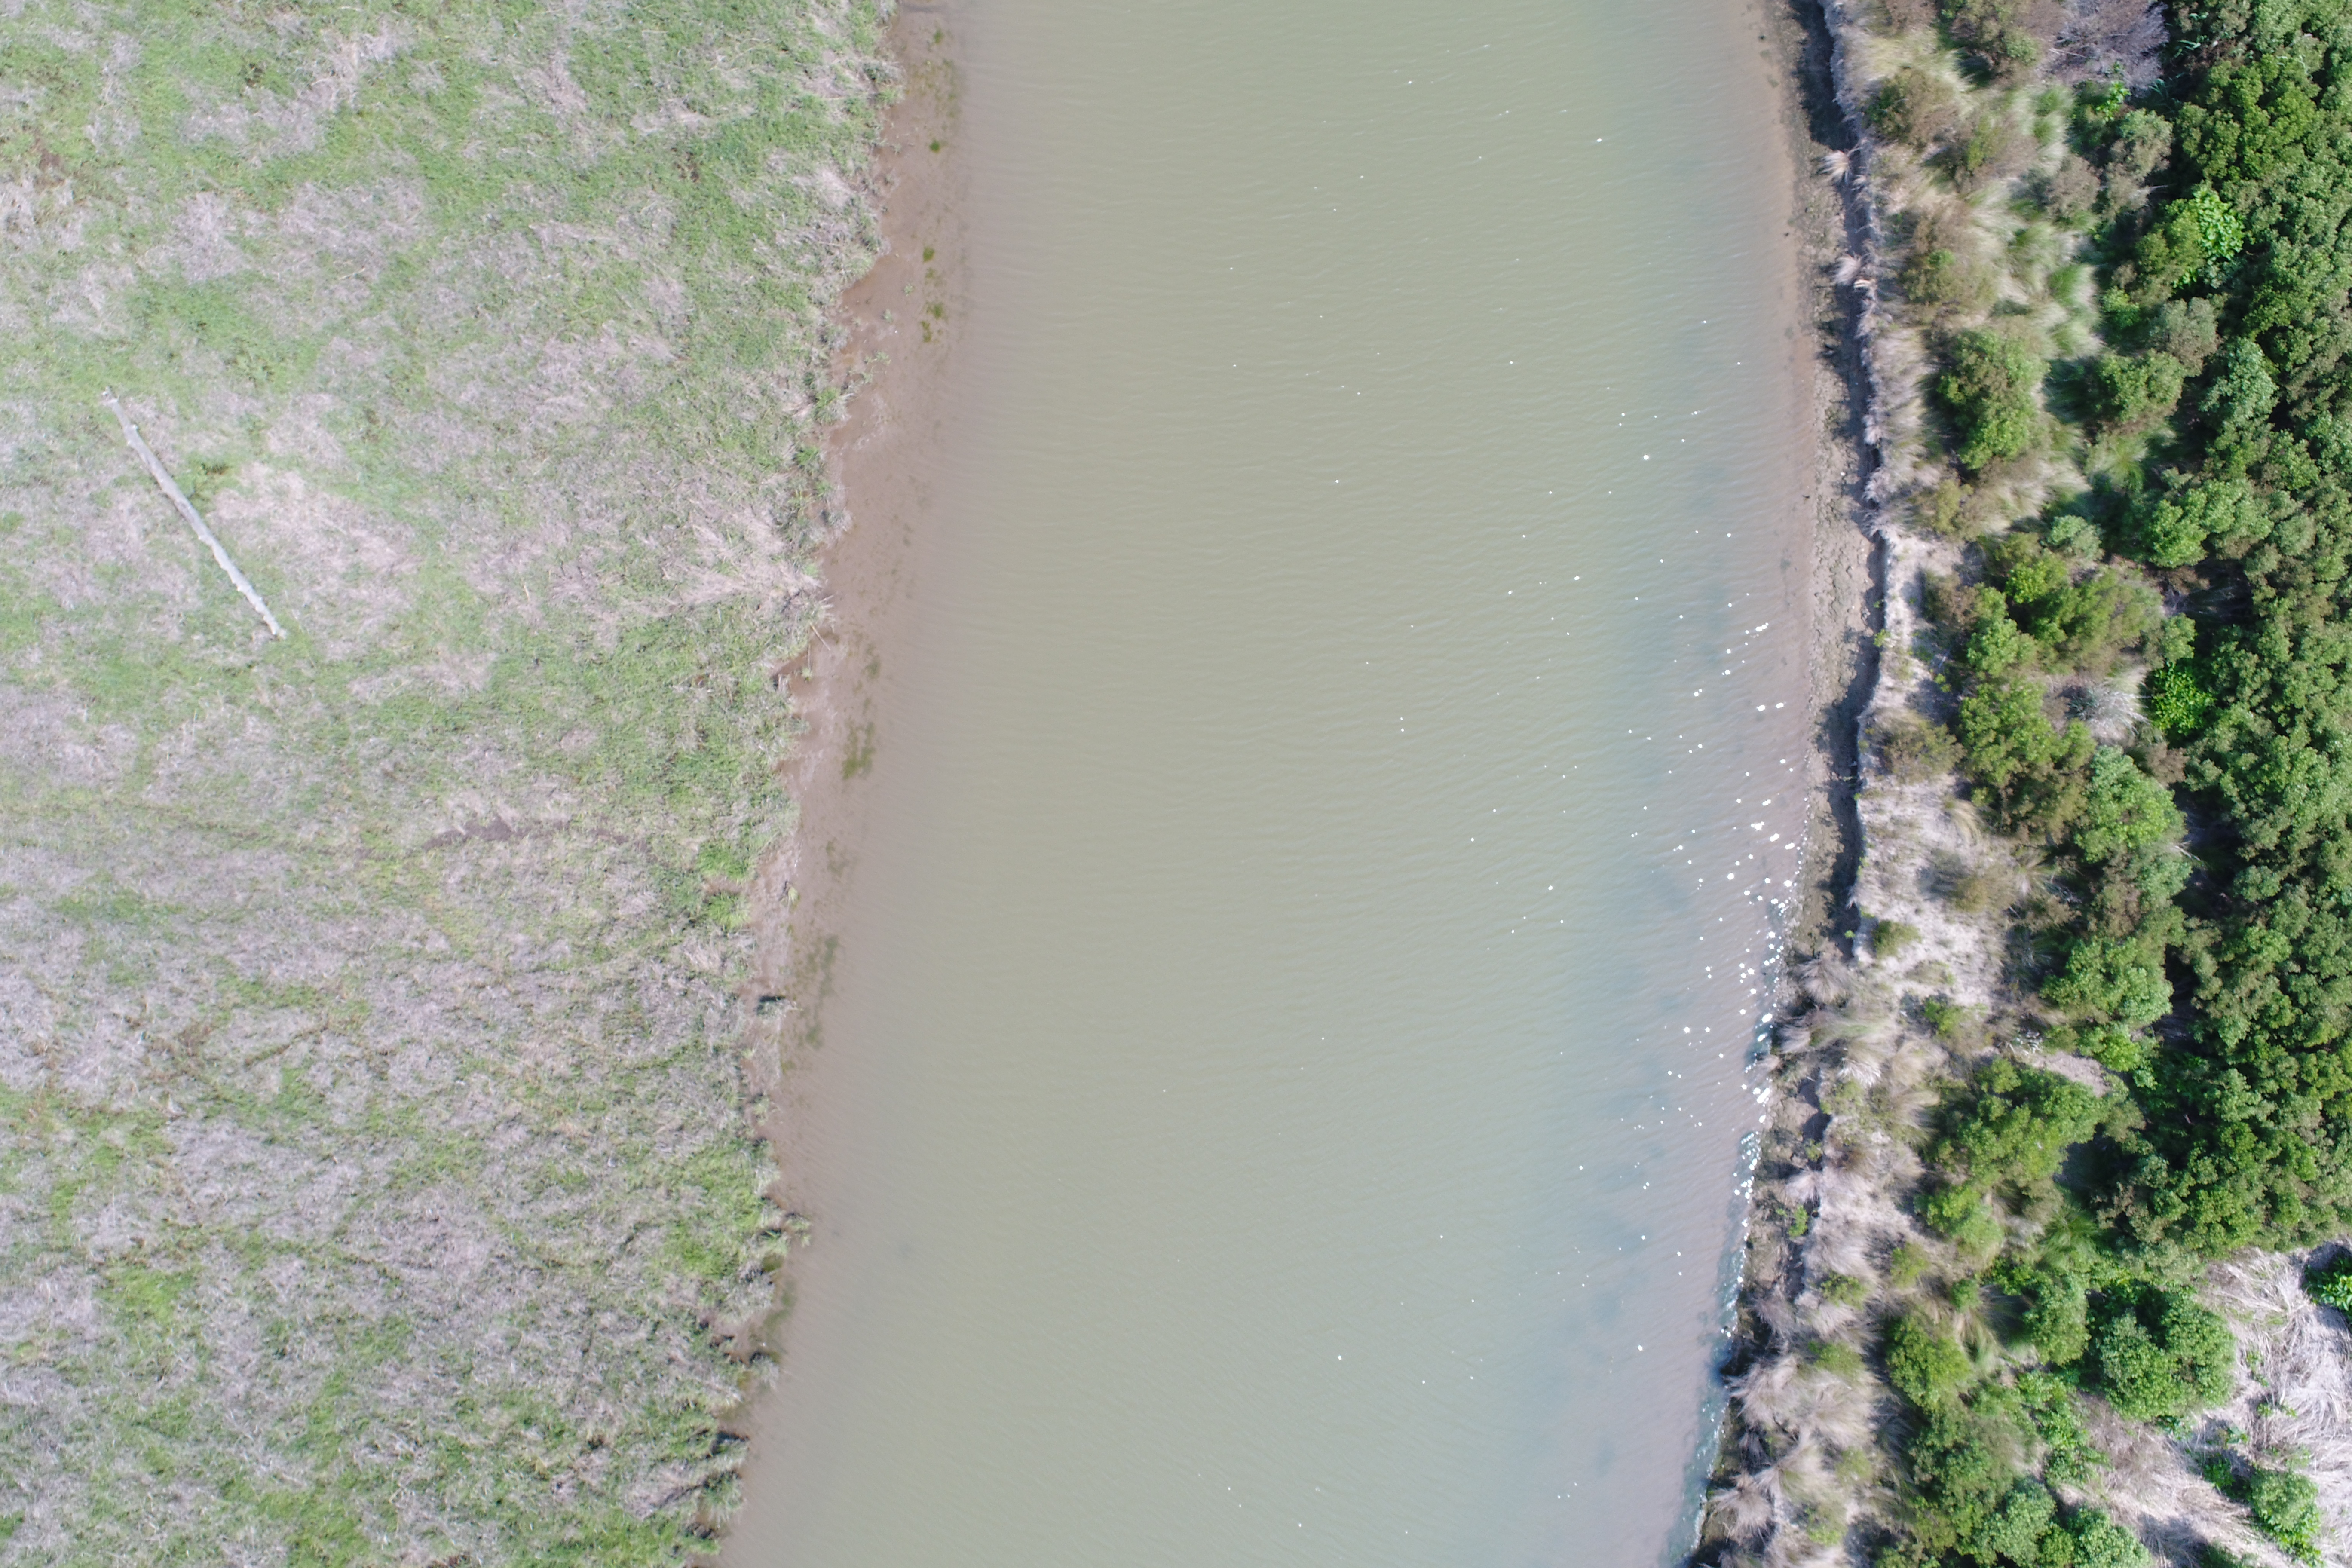
\includegraphics[width=\textwidth]{images/site_poplar_island_aerial.JPG} \\
        (a)
    \end{minipage}\hfill
    \begin{minipage}[b]{0.48\textwidth}
        \centering
        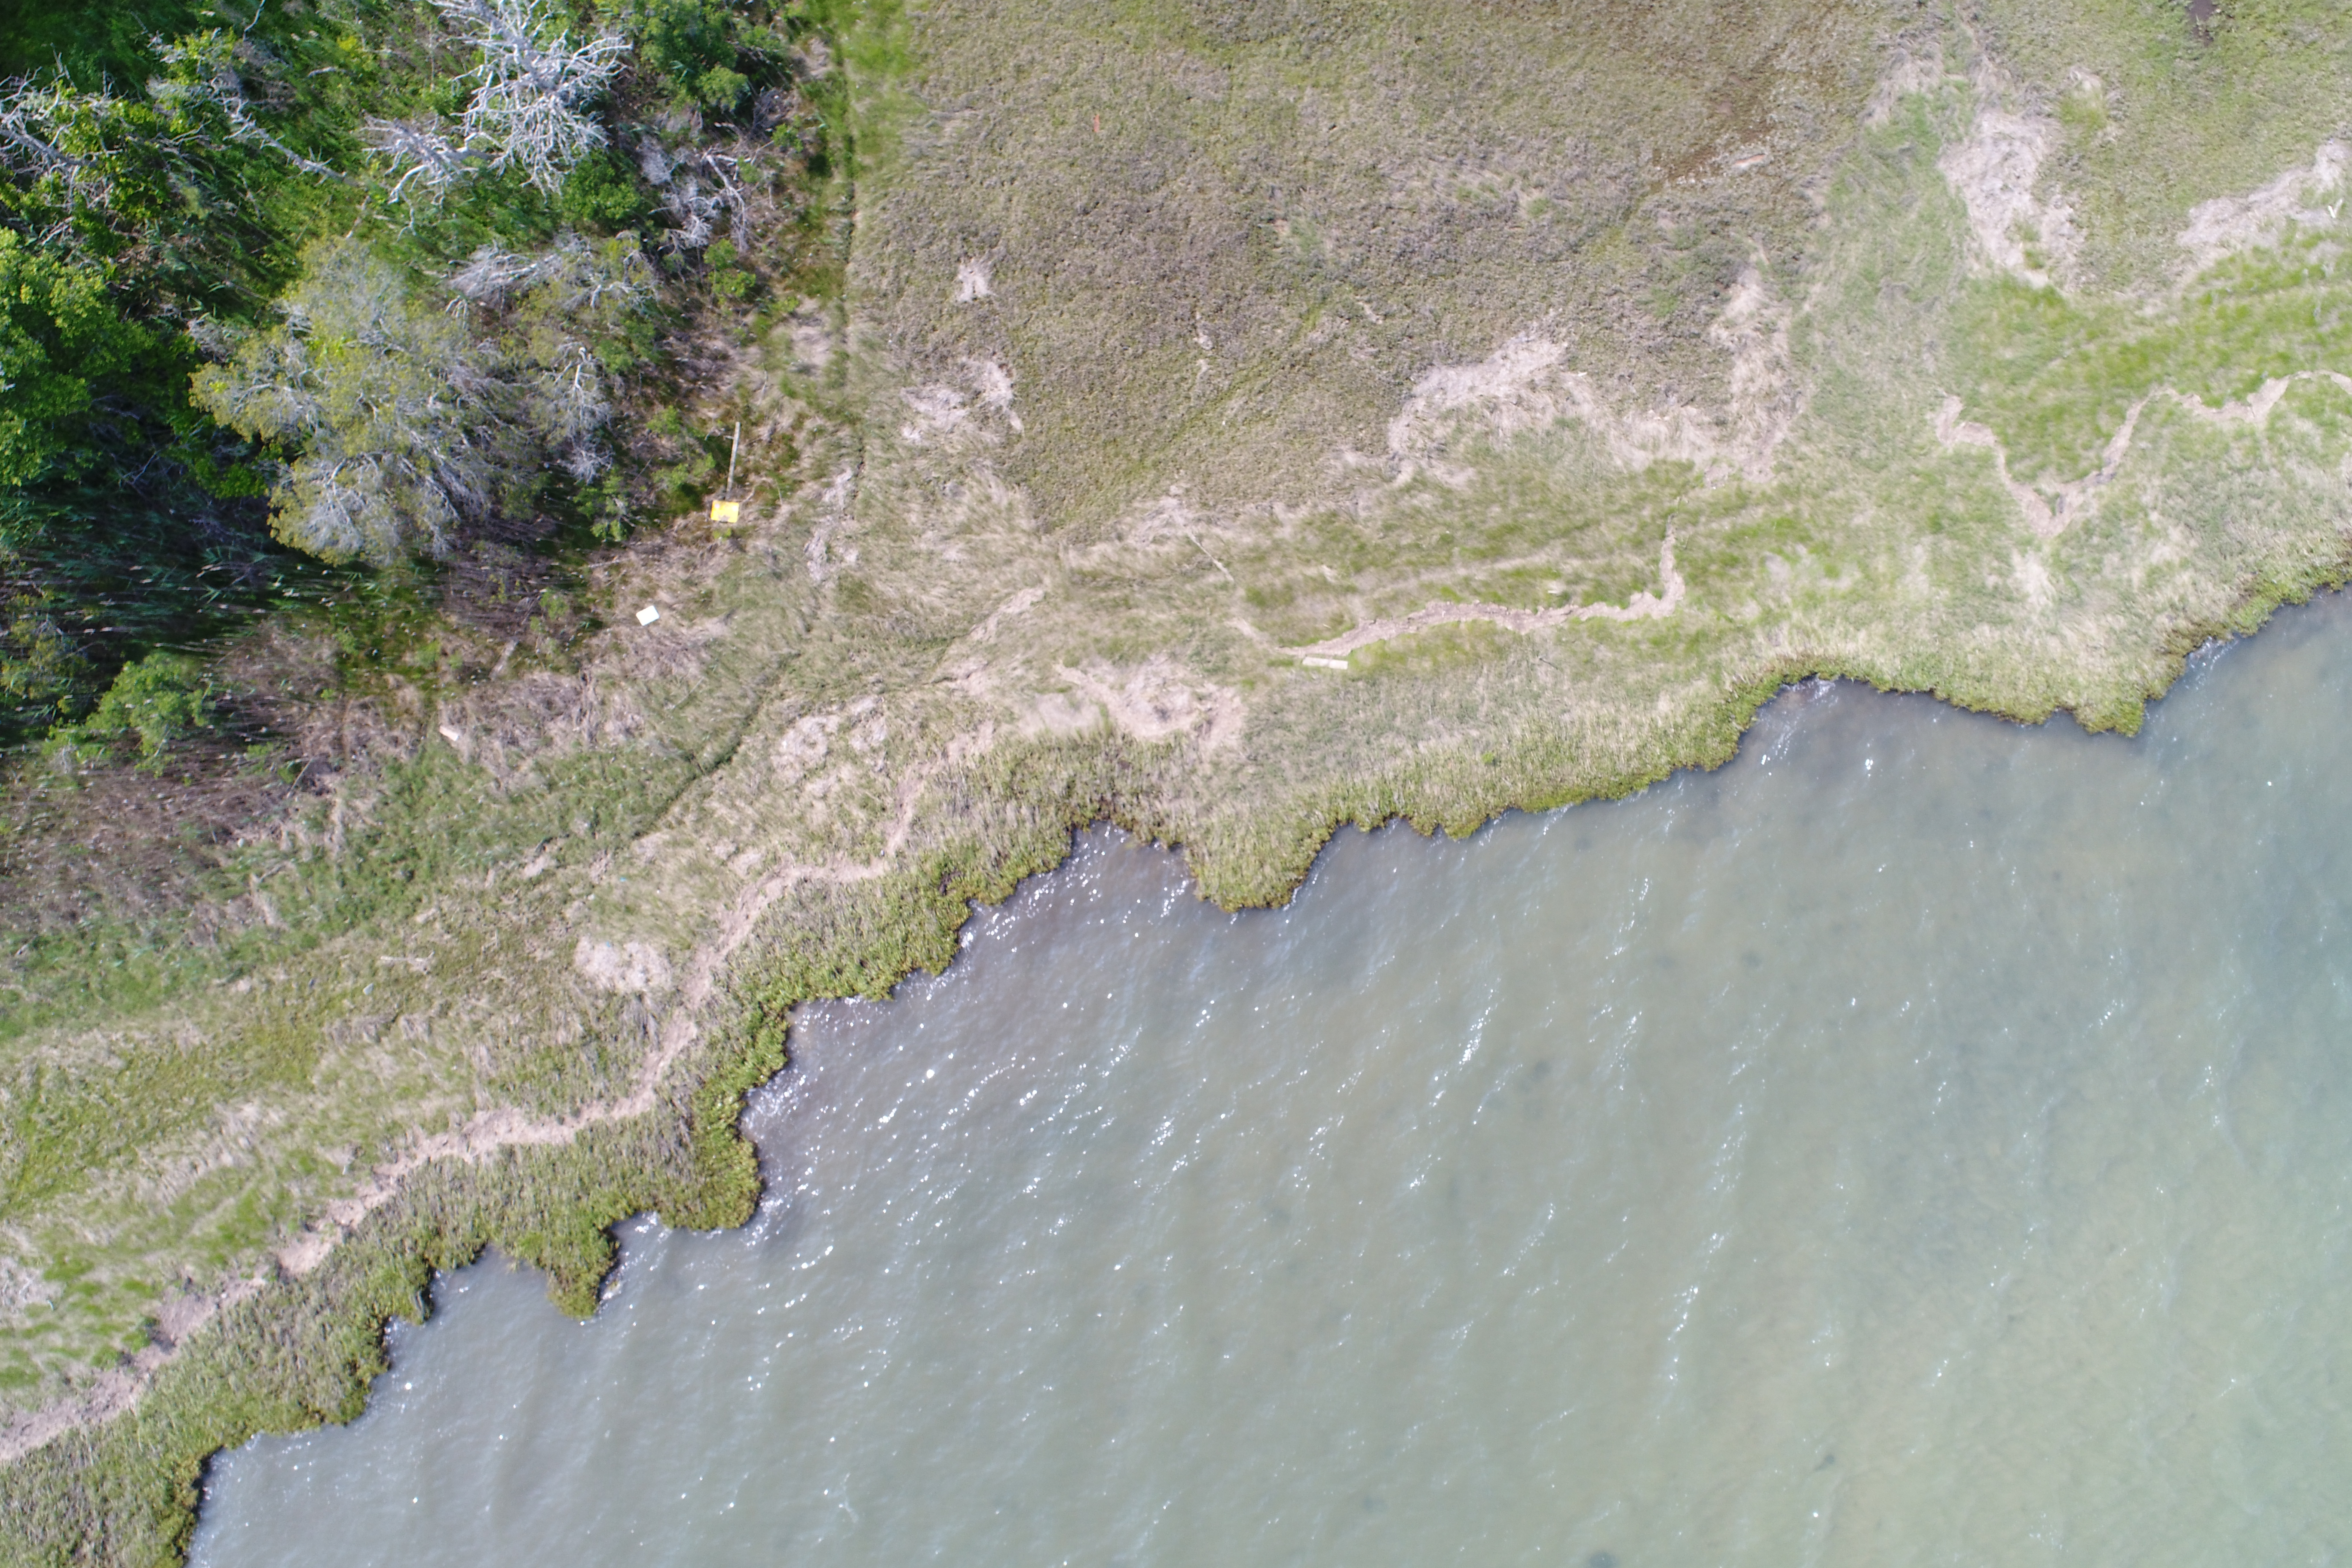
\includegraphics[width=\textwidth]{images/site_assateague_island_aerial.JPG} \\
        (b)
    \end{minipage}
    
    \vspace{1em} % spazio verticale tra le righe

    % Seconda riga: (c) + (d) in alto a sinistra del quarto quadrante
    \begin{minipage}[t]{0.48\textwidth} % <<< Usa [t] per allineare in alto
        \centering
        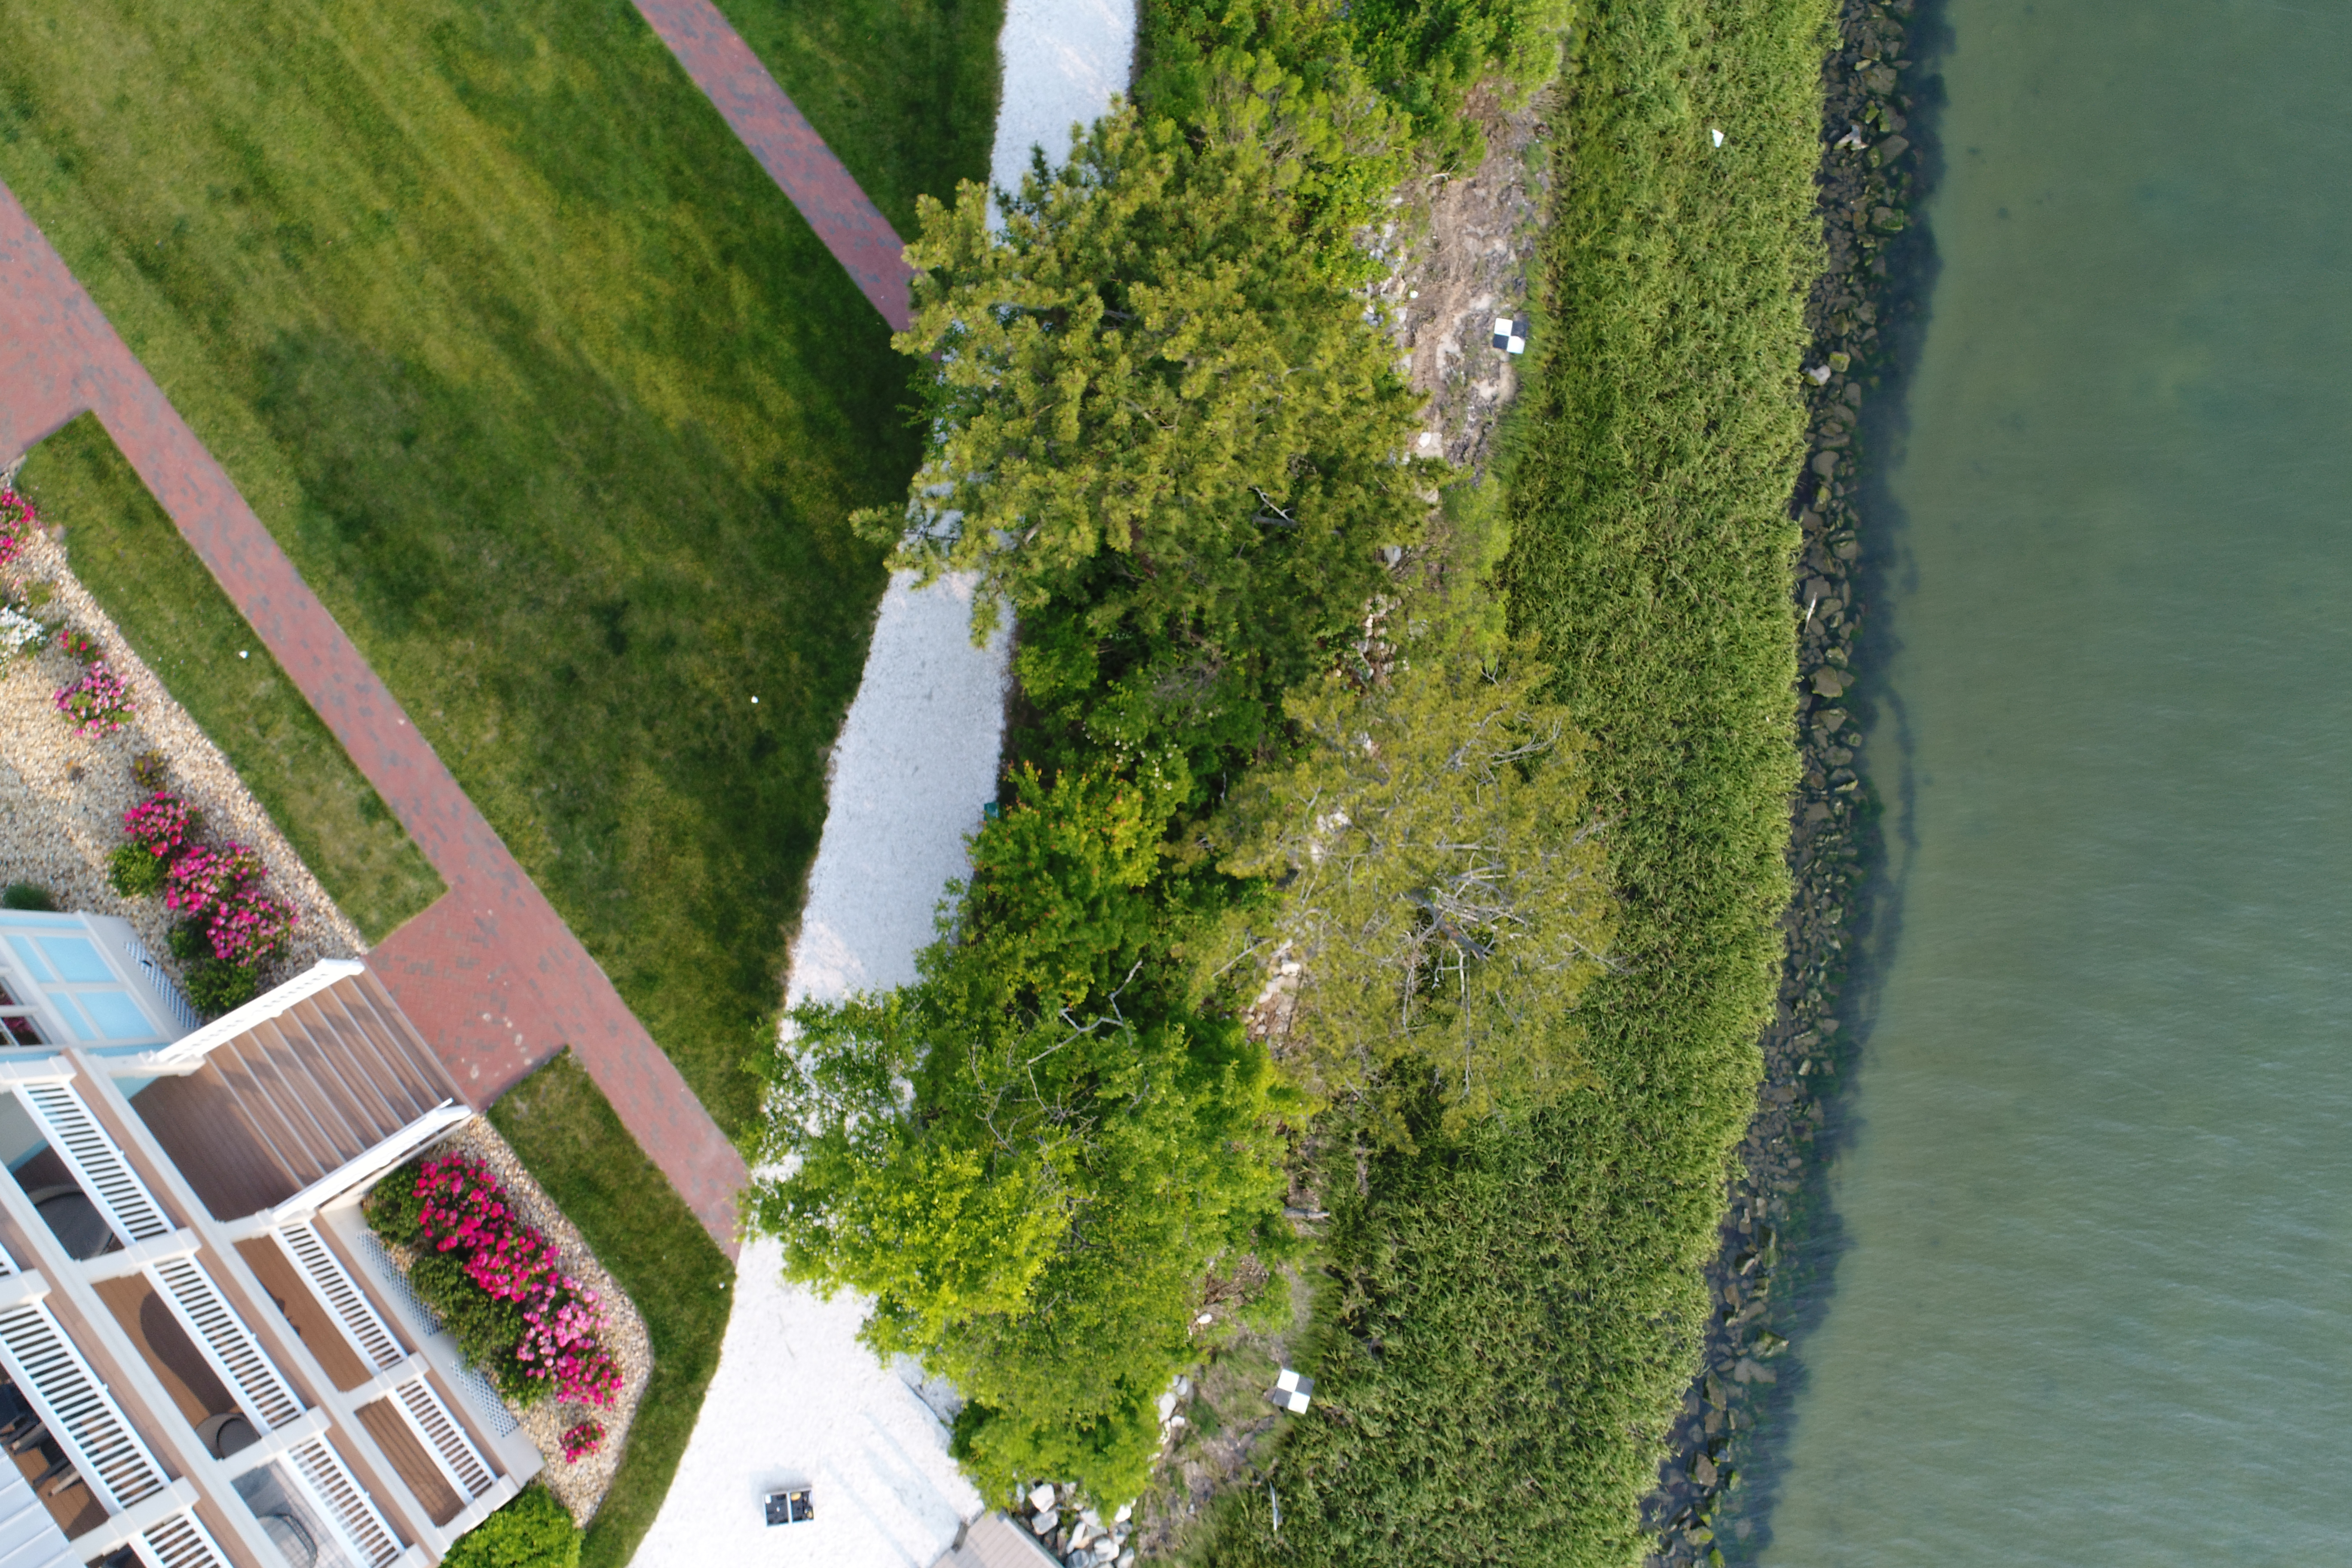
\includegraphics[width=\textwidth]{images/site_sunset_island_aerial.JPG} \\
        (c)
    \end{minipage}\hfill
    \begin{minipage}[t]{0.48\textwidth} % <<< Anche qui [t]
        \raggedright % <<< Allinea a sinistra dentro lo spazio
        \includegraphics[width=0.6\textwidth]{images/study_area_chesapeake_bay_map.png} \\
        (d)
    \end{minipage}

    \caption{Representative aerial images of the study sites: (a) Poplar Island, (b) Assateague Island, (c) Sunset Island, and (d) geographic context within the Chesapeake Bay region. Note: Map lines delineate study areas and do not necessarily depict accepted national boundaries.}
    \label{fig:siti}
\end{figure}

\subsubsection{UAV Image Acquisition}

The dataset was developed using high-resolution imagery acquired during low-altitude UAV surveys conducted over Poplar Island, Assateague Island, and Sunset Island (Maryland, USA) in December 2024. Aerial data collection consisted of four distinct flight missions per site, covering approximately 400 m × 400 m of surface area.
All flights were carried out using a DJI Phantom 3 Professional (DJI-P3P) drone equipped with two sensors: the integrated DJI FC300X RGB camera and an additional multispectral camera. The flight plans were created using the Pix4D Capture application, with key parameters set to longitudinal overlap 80\%, lateral overlap 60\% and constant flight altitude of 40 meters. These settings ensured complete and consistent spatial coverage, minimizing gaps between adjacent flight lines. The additional multispectral payload reduced the drone’s flight autonomy, a factor considered during mission planning. The RGB imagery collected by the FC300X sensor achieved a Ground Sample Distance (GSD) of approximately 1.8 cm, while the multispectral imagery obtained a GSD of around 2.8 cm. These values were computed based on sensor specifications, pixel size, focal length, and flight altitude, ensuring high spatial resolution suitable for fine-scale environmental analyses.

The resulting imagery, encompassing a variety of coastal and wetland environments—including marshland, small watercourses, and vegetated areas—was used to build a texture-based dataset. Representative samples of key environmental classes were manually extracted from the images. The annotation process was implemented through a Python workflow involving the extraction and labeling of 128×128 pixel patches from the orthomosaics. For each class, 40 patches per site were selected, resulting in the creation of a `clean' dataset composed of high-quality manually annotated samples. The images are in 8-bit per channel RGB PNG format.

\subsection{Classification Dataset and Data Organization}

The overall dataset is organized by geographic area, with each site characterized by specific land cover classes: low\_veg (low vegetation): areas characterized by herbaceous vegetation, grasses, and low-height plant cover typical of marshland and coastal meadows; trees (trees/woody vegetation): areas with tree cover, forests, and significant woody vegetation; water: present in Poplar and Assateague, includes water bodies, tidal channels, and flooded wetlands; garden: present only in Sunset, representing anthropogenic green areas, residential gardens, and ornamental vegetation
This organization reflects the different ecological characteristics of the sites: Poplar and Assateague include extensive natural aquatic environments (tidal marshes and channels), while Sunset, being a residential urban area, presents anthropogenic elements such as gardens instead of natural water zones.
The adopted naming convention follows the consistent pattern:
\texttt{\{noise\_type\}\_\{noise\_intensity\}\_\{dataset\allowbreak\_dimension\}\_\{location\}},
where \texttt{noise\_type} identifies the type of noise and \texttt{intensity} the numerical parameter controlling its strength.
Further details on the rationale behind the selection of the noise types, along with a brief description of each, are provided in the Supplementary Materials section.

\subsubsection{Dataset dimension differentiation} 
To investigate the effect of dataset size on model performance, three size variants were created: Mini, $\sim$5 images per class (total $\sim$15 images), used to test extreme data scarcity scenarios; Small, $\sim$10 images per class (total $\sim$30 images), representative of scenarios with moderate data limitation; Original, $\sim$40 images per class (total $\sim$120 images), constituting the full available dataset
An Augmented variant was also prepared ($\sim$100 images per class, total $\sim$300 images) using data augmentation techniques (rotations at $90^\circ$, $180^\circ$, $270^\circ$ and horizontal/vertical flips). However, preliminary tests revealed that the improvement in accuracy from the Original dataset to the Augmented dataset was negligible (increase $<1\%$), suggesting that the Original dataset  already represents a plateau point in the learning curve. Therefore, the Augmented dataset was excluded from the systematic experimental suite to optimize computational efficiency without compromising the scientific validity of the study.

\subsubsection{Synthetic noise differentiation} 
To evaluate the robustness of feature extraction methods under non-ideal operating conditions, the clean dataset was systematically corrupted with five types of noise, each tested at three intensity levels (low, moderate, high), for a total of 15 corrupted dataset variants plus the clean baseline dataset. The noise types were selected to represent different sources of signal degradation commonly encountered in remote sensing and UAV imaging applications and a summary is available in Table~\ref{tab:noise_summary}.

\begin{table}[t]
    \centering
    \caption{Noise Dataset Summary}
    \label{tab:noise_summary}
    \begin{tabular}{l c c c c}
        \toprule
        \textbf{Noise Type} & \textbf{Low Level} & \textbf{Moderate Level} & \textbf{High Level} & \textbf{Total Variants} \\
        \midrule
        \textbf{Gaussian} & - & $\sigma=30$ & $\sigma=50$ & 2 \\
        \textbf{Poisson} & - & $\lambda=60$ & $\lambda=100$ & 2 \\
        \textbf{Salt \& Pepper} & 5\% & 15\% & 25\% & 3 \\
        \textbf{Speckle} & $\sigma^2=15$ & $\sigma^2=35$ & $\sigma^2=55$ & 3 \\
        \textbf{Uniform} & $r=10$ & $r=25$ & $r=40$ & 3 \\
        \textbf{Clean} & -- & -- & -- & 1 \\
        \midrule
        \textbf{TOTAL} & & & & \textbf{14 datasets} \\
        \bottomrule
    \end{tabular}
\end{table}

\subsection{Feature Extraction and Feature Selection}
The extraction of features from RGB images represents the critical step for transforming raw data into a numerical representation suitable for machine learning. Three distinct methodological approaches were implemented and compared: a first method, considered to be the standard approach, consisted in the extraction of statistical descriptors from RGB images and was carried out by computing 18 features for each channel, for a total of 54 features. These include first-order statistics, distribution shape indicators, robust quantile-based measures, and spatial texture features. The complete set of features is reported in Table~\ref{tab:stat_features}.

\subsubsection{Wavelet Scattering Transform (WST)} 
The second approach involves the Wavelet Scattering Transform \cite{Bruna2013Invariant}, which is a multi-scale, translation-invariant representation that extends the wavelet transform through cascades of wavelet modulus operators and nonlinearities. Unlike convolutional neural networks, WST does not require filter learning, as it relies on predefined Morlet wavelets across multiple orientations and scales.
The scattering operator $S$ is defined recursively:

\begin{align}
    \textbf{Order 0:} & \quad S_0 x = x \star \varphi_J \\
    \textbf{Order 1:} & \quad S_1 x(\lambda_1) = |x \star \psi_{\lambda_1}| \star \varphi_J \\
    \textbf{Order 2:} & \quad S_2 x(\lambda_1, \lambda_2) = ||x \star \psi_{\lambda_1}| \star \psi_{\lambda_2}| \star \varphi_J
\end{align}

where $\varphi_J$ is a low-pass filter (father wavelet) at scale $J$, $\psi_{\lambda}$ are Morlet wavelets parameterized by $\lambda = (j, \theta)$ with scale $j$ and orientation $\theta$, $\star$ denotes the convolution operation, $|\cdot|$ is the complex modulus (non-linearity)
We employ the Kymatio library \cite{andreux2020kymatio}, which provides an efficient implementation of the WST.
The WST generates scattering coefficients for each channel, producing approximately 81 scattering coefficients per channel; from these, mean and standard deviation statistics are computed, for a total of $\sim162$ features per channel, and a total of $\sim486$ WST features on the RGB image. These capture multi-scale spatial information (from fine textures to coarse patterns), are invariance to small translations and deformations and are discriminative of directional orientations. The advantages of WST are  the invariance, showing to be robust to small deformations and translations, stability of the coefficients, interpretability thanks to wavelet filters with clear geometric meaning and no need for training due to the fact that no parameter learning is needed.

The hybrid approach combines the 54 Advanced Statistical Features with the WST features, leveraging the complementarity of the two representations by capturing pointwise statistical properties and intensity distributionsbut also spatial patterns, textures, and multi-scale structures. The combination provides a rich representation that benefits both from the interpretability of statistical descriptors and the ability of WST to capture complex patterns.

Regardless of the extraction method, all features were normalized using scikit-learn's \texttt{StandardScaler} \cite{scikit-learn}. 
\[
z = (x - \mu) / \sigma
\]
where $\mu$ and $\sigma$ are computed on the training set and applied to both training and test sets to avoid data leakage \cite{scikit-learn}.

\begin{table}[t]
    \centering
    \caption{Complete set of statistical features (18 per RGB channel, 54 total).}
    \label{tab:stat_features}
    \begin{tabular}{p{3cm} p{4cm} p{8cm}}
        \toprule
        \textbf{Category} & \textbf{Feature} & \textbf{Description} \\
        \midrule
        Basic Statistics & Mean ($\mu$) & Central value of the intensity distribution \\
         & Standard Deviation ($\sigma$) & Dispersion of intensity values \\
         & Variance ($\sigma^2$) & Square of the standard deviation \\
         & Minimum & Lowest pixel intensity in the channel \\
         & Maximum & Highest pixel intensity in the channel \\
         & Range & Difference between maximum and minimum values \\
        \midrule
        Shape Statistics & Skewness & Asymmetry of the distribution relative to the mean \\
         & Kurtosis & Tail weight relative to a normal distribution \\
         & Coefficient of Variation (CV) & Normalized dispersion: $\sigma / \mu$ \\
        \midrule
        Robust/Percentile Stats & 10th Percentile & Lower quantile of the intensity distribution \\
          & 25th Percentile & First quartile of the intensity distribution \\
          & Median (50th) & Central value less sensitive to outliers \\
          & 75th Percentile & Third quartile of the intensity distribution \\
          & 90th Percentile & Upper-tail quantile \\
          & Interquartile Range (IQR) & Difference between 75th and 25th percentile \\
          & Median Absolute Deviation (MAD) & Median of absolute deviations from the median \\
        \midrule
        Spatial Features & Gradient Mean & Mean spatial gradient (Sobel-based) \\
         & Edge Density & Percentage of edge pixels (Laplacian thresholding) \\
        \bottomrule
    \end{tabular}
\end{table}

\subsubsection{Features Selection} 
Given the high dimensionality of the feature space, a feature selection phase was applied to identify the most informative subset and reduce the risk of overfitting. The SelectKBest algorithm from scikit-learn was used, with scoring based on Mutual Information (MI). Mutual information measures the non-linear dependency between each feature $X_i$ and the target variable $Y$:
\[
\text{MI}(X_i; Y) = \sum_{x_i} \sum_{y} p(x_i, y) \log\left(\frac{p(x_i, y)}{p(x_i)p(y)}\right)
\]
where $p(x_i, y)$ is the joint distribution and $p(x_i)$ and $p(y)$ are the marginal distributions
Mutual information offers significant advantages over linear methods such as Pearson correlation, as it captures non-linear dependencies, does not assume a Gaussian distribution, is invariant under monotonic transformations, and has a range of $[0, \infty]$, with $0$ indicating independence \cite{scikit-learn}.
Four values,  2, 5, 10, 20 of $k$ were systematically tested. Experimental analysis revealed that \textbf{$k=5$} provides the best compromise between accuracy (0.930) and model complexity. Feature selection is always performed on the training set and applied to the test set to avoid selection bias.

\subsection{Classification through Random Forest}

Random Forest \cite{Breiman2001} is an ensemble learning method that constructs multiple decision trees during training and outputs the modal class (classification) or the mean prediction (regression) of the individual trees.
For each tree $t$ in the ensemble, a bootstrap sample is first drawn from the training set (bagging), and at every split only a random subset of $\sqrt{p}$ out of the $p$ available features is considered; the tree is then grown to full depth (or until other stopping criteria are met), and the final prediction is obtained by majority voting across all trees.
Among the reasong of Random Forest choice are reduced variance compared to individual decision trees, robustness to overfitting, natural handling of non-linear features and interactions, the ability to provide feature importance, and inherent parallelizability.
The Random Forest model was configured with an adaptive setup, where the number of trees was scaled according to the size of the dataset. All hyperparameters used in the experiments are summarized in Table~\ref{tab:rf_hyperparams}.
The rationale behind \texttt{n\_estimators} is that the number of trees was scaled proportionally to the size of the training set to balance generalization capacity and computational cost. Smaller datasets are more prone to overfitting with many trees, whereas larger datasets benefit from additional trees that improve prediction stability.

\begin{table}[t]
    \centering
    \caption{Random Forest hyperparameters and configuration details.}
    \label{tab:rf_hyperparams}
    \begin{tabular}{p{4cm} p{9cm}}
    \toprule
    \textbf{Hyperparameter} & \textbf{Value / Description} \\
    \midrule
    \textbf{n\_estimators} & Mini: 3 trees; Small: 10 trees; Original: 50 trees \\
    \textbf{criterion} & Gini impurity \\
    \textbf{max\_depth} & None (trees grown until pure leaves) \\
    \textbf{min\_samples\_split} & 2 \\
    \textbf{min\_samples\_leaf} & 1 \\
    \textbf{max\_features} & \texttt{sqrt} ($\sqrt{p}$ features considered at each split) \\
    \textbf{bootstrap} & True \\
    \textbf{random\_state} & 42 (for reproducibility) \\
    \bottomrule
    \end{tabular}
\end{table}

\subsubsection{Model Validation} The dataset was partitioned into 5 folds while ensuring that class proportions were maintained in each split. The 5-fold Stratified Cross-Validation procedure was applied throughout the training of all 1 512 Random Forest models. This approach helps produce a more stable estimate of expected model performance by mitigating the variability associated with any single train/test partition. Indeed, multiple studies apply a similar stratified CV methodology in related domains \cite{witten2016valutazione, kohavi1995crossvalidation, szeghalmy2023scv}.
The procedure divides the data into 5 disjoint subsets (folds) and conducts 5 rounds of validation: in each round, 4 folds (80\% of the data) serve as the training set, and the remaining fold (20\%) is used for validation. The stratified component ensures that the class distribution in each fold mirrors that of the full dataset, which is especially valuable when working in low-data regimes (e.g. the “mini” setting). Without stratification, some classes might be over- or under-represented in certain folds, biasing the evaluation.
We store in each experiment’s JSON output the cross-validation metrics (\texttt{cv\_mean\_accuracy}, \texttt{cv\_std\_accuracy}, \texttt{cv\_scores}), which tend to be more robust than a single train/test measurement. Averaging across folds reduces dependence on particularly favorable or unfavorable splits. The standard deviation across folds (\texttt{cv\_std}) also offers insight into model stability: small values (e.g. < 0.02) suggest consistency across partitions, while larger ones (e.g. > 0.05) may indicate sensitivity to splits, overfitting, or insufficient sample size.
Lastly, the final Train/Test partition is set at 80\% training and 20\% testing. Stratification is preserved via \texttt{stratify = y} to maintain consistency in class proportions across both subsets.

\subsubsection{Evaluation Metrics}
The following metrics were computed for each experiment:

\textbf{Accuracy}:
\[
\text{Acc} = \frac{\text{TP} + \text{TN}}{\text{TP} + \text{TN} + \text{FP} + \text{FN}}
\]
Proportion of correct predictions over the total. Appropriate given the class balance (1:1:1 ratio).

\textbf{Precision (per class)}:
\[
\text{Prec} = \frac{\text{TP}}{\text{TP} + \text{FP}}
\]
Proportion of correctly predicted positive samples. Measures the classifier’s specificity.

\textbf{Recall (per class)}:
\[
\text{Rec} = \frac{\text{TP}}{\text{TP} + \text{FN}}
\]
Proportion of actual positives that are correctly identified. Measures the classifier’s sensitivity.

\textbf{F1-Score (per class)}:
\[
\text{F1} = 2 \cdot \frac{\text{Prec} \cdot \text{Rec}}{\text{Prec} + \text{Rec}}
\]
Harmonic mean of precision and recall, providing a balanced single metric.

\textbf{Confusion Matrix}:\\
Matrix $C$ where $C_{ij}$ represents the number of samples from class $i$ predicted as class $j$. Enables a detailed analysis of misclassification patterns.

\textbf{Cross-Validation Metrics}: CV Mean Accuracy across the 5 folds and CV standard deviation of accuracy (indicator of stability)

The choice of metrics—accuracy, precision, recall, F1-score, confusion matrix, and cross-validation indicators—is motivated by their established roles in providing a comprehensive assessment of classification performance, capturing distinct aspects such as overall correctness, specificity, sensitivity, and robustness to class imbalance. The combination of class-level and aggregate metrics allows for a more detailed interpretation, while cross-validation ensures statistical reliability across multiple dataset partitions \cite{witten2016valutazione,Powers2011}.

\subsection{Statistical Analysis}
The specific objectives of the statistical analysis are:
\begin{enumerate}
    \item \textbf{Quantify comparative robustness} under 6 noise types (Gaussian, Poisson, Salt\&Pepper, Speckle, Uniform) at increasing intensities
    \item \textbf{Evaluate data efficiency} in scenarios of extreme scarcity (mini: $\sim5$ img/class), moderate (small: $\sim15$ img/class), and standard (original: $\sim40$ img/class)
    \item \textbf{Determine specific configurations} (noise type $\times$ intensity $\times$ dataset size $\times k$-features) where WST or Hybrid show statistically significant advantages
    \item \textbf{Separate statistical significance from practical relevance} through effect size analysis
\end{enumerate}
To rigorously evaluate the comparative robustness of the feature extraction methods (Advanced Statistics, WST, Hybrid), non-parametric statistical tests were applied with correction for multiple comparisons, effect size calculation, and control for spatial autocorrelation through geographic aggregation. The analysis was designed to separate statistical significance from practical relevance and identify specific configurations where each method shows advantages.

\subsubsection{Dataset Construction and Full Factorial Experimental Design}
The experimental dataset consists of a fully crossed factorial design yielding a total of $1512$ individual experiments. Each experiment is defined by a unique combination of six independent factors: geographic area, dataset size, feature extraction method, K-best dimensionality, noise type, and noise intensity. 
The base factorial grid consists of:
\[3 
\text{ areas} \times 3 \text{ sizes} \times 3 \text{ feature methods} \times 
4 \text{ K-values} = 108 \text{ base configurations.}
\]
Each of these 108 configurations was expanded according to the six noise families and their associated intensity levels (Table~\ref{tab:noise_intensities}). This resulted in:
\begin{itemize}
    \item Clean: $108 \times 1 = 108$
    \item Gaussian: $108 \times 2 = 216$ ($\sigma = 30, 50$)
    \item Poisson: $108 \times 2 = 216$ ($\lambda = 40, 60$)
    \item Salt \& Pepper: $108 \times 3 = 324$ ($p = 5\%, 15\%, 25\%$)
    \item Speckle: $108 \times 3 = 324$ ($\sigma^2 = 15, 35, 55$)
    \item Uniform: $108 \times 3 = 324$ ($r = 10, 25, 40$)
\end{itemize}
Table~\ref{tab:dataset_factors_unified} summarizes all factors in the factorial design.
Noise models and their controlled intensity levels are reported in 
Table~\ref{tab:noise_intensities}. These parameters were used to generate corrupted versions of the clean orthomosaics for all three geographical locations.
To guarantee full reproducibility of the experimental pipeline, every potential source of randomness was explicitly controlled. All random number generators were initialized with fixed seeds (\texttt{Python}=42, \texttt{NumPy}=42, and \texttt{scikit-learn} components using \texttt{random\_state=42}), ensuring that dataset splits, noise generation, and classifier behavior followed identical sequences across repeated runs. In addition, the order of all processing steps was kept strictly fixed, and each experimental configuration was saved in a dedicated JSON file. This deterministic setup ensures that the complete sequence of operations can be replicated exactly, both within this study and in future extensions.
To reduce spatial autocorrelation and obtain robust performance estimates, results from the three geographic areas were averaged. For each configuration, the mean and standard deviation of each metric were computed across the three locations.
This aggregation reduces the $1512$ raw experiments into $504$ configuration-level observations used for statistical analysis.
Table~\ref{tab:evaluation_metrics} lists the metrics extracted from each experimental run.

\begin{table}[t]
    \centering
    \caption{Summary of the factors defining the full experimental dataset.}
    \label{tab:dataset_factors_unified}
    \begin{tabular}{llc}
        \toprule
        \textbf{Factor} & \textbf{Values} & \textbf{Levels} \\
        \midrule
        Geographic Areas & Assateague, Poplar, Sunset & 3 \\
        Dataset Sizes & mini ($\sim$5 img/class), small ($\sim$15), original ($\sim$40) & 3 \\
        Feature Methods & advanced\_stats, wst, hybrid & 3 \\
        K-best Values & 2, 5, 10, 20 & 4 \\
        Noise Types & clean, gaussian, poisson, saltpepper, speckle, uniform & 6 \\
        Noise Intensities & See Table~\ref{tab:noise_intensities} & -- \\
        Land Cover Classes & 3 per area (Sunset: garden replaces water) & -- \\
        \bottomrule
    \end{tabular}
\end{table}

\begin{table}[t]
    \centering
    \caption{Noise families and intensity levels used to generate corrupted dataset variants.}
    \label{tab:noise_intensities}
    \begin{tabular}{lcl}
        \toprule
        \textbf{Noise Type} & \textbf{Intensity Levels} & \textbf{Parameters} \\
        \midrule
        Clean & 1 & No corruption \\
        Gaussian & 2 & $\sigma = 30, 50$ \\
        Poisson & 2 & $\lambda = 40, 60$ \\
        Salt \& Pepper & 3 & $p = 5\%, 15\%, 25\%$ \\
        Speckle & 3 & $\sigma^2 = 15, 35, 55$ \\
        Uniform & 3 & $r = 10, 25, 40$ \\
        \bottomrule
    \end{tabular}
\end{table}

\begin{table}[t]
    \centering
    \caption{Performance metrics extracted for each of the 1,512 experiments.}
    \label{tab:evaluation_metrics}
    \begin{tabular}{lp{9cm}}
        \toprule
        \textbf{Metric} & \textbf{Description} \\
        \midrule
        Test Accuracy & Computed on the 20\% hold-out test set \\
        Macro-averaged F1-score & Weighted harmonic mean of Precision and Recall over the 3 classes \\
        Macro-averaged Precision & Average class-wise Precision, unweighted by class frequency \\
        Macro-averaged Recall & Average class-wise Recall, unweighted by class frequency \\
        Cross-validation Scores & 5-fold stratified CV accuracy values (mean and standard deviation) \\
        Confusion Matrix & $3 \times 3$ matrix showing class-wise prediction distribution \\
        \bottomrule
    \end{tabular}
\end{table}

\subsection{Structure of the Analytical Framework} 

\subsubsection{Pairwise Comparisons Between Methods} 
To quantify the relative differences between methods in a statistically rigorous way, pairwise deltas were calculated for each configuration.
For each configuration $i \in \{1, \ldots, 168\}$ (after removing the location effect and aggregating on intensity for some analyses):
\[
\begin{aligned}
    \Delta_{\text{WST},i} &= \text{Macro-F1}_{\text{WST}}(i) - \text{Macro-F1}_{\text{AdvStats}}(i) \\
    \Delta_{\text{Hybrid},i} &= \text{Macro-F1}_{\text{Hybrid}}(i) - \text{Macro-F1}_{\text{AdvStats}}(i)
\end{aligned}
\]

Where Advanced Stats is the common baseline.
The Comparisons Performed are:

\[
\begin{aligned}
    \textbf{WST vs Adv. Stats} &= \text{WST} - \text{AdvStats} \\
    \textbf{Hybrid vs Adv. Stats} &= \text{Hybrid} - \text{AdvStats}
\end{aligned}
\]

For each combination of noise type, intensity level, dataset size, and $k$ value, performance deltas were computed by comparing alternative feature extraction methods against the Advanced Statistical Features baseline. In total, 168 deltas were calculated for WST vs.\ AdvStats and an additional 168 deltas for Hybrid vs.\ AdvStats, resulting in 336 pairwise comparisons.
A positive delta ($\Delta > 0$) indicates that the tested method outperforms Advanced Stats, whereas a negative delta ($\Delta < 0$) suggests inferior performance relative to the baseline. Values close to zero imply equivalent effectiveness between the two approaches.
Aggregating the deltas across all configurations enables a quantitative assessment of both average performance differences and their variability. Specifically:
the expected value $\mathbb{E}[\Delta]$ reflects the average effect of switching from AdvStats to an alternative method; the standard deviation $\text{Std}[\Delta]$ captures the consistency of this effect (with lower values indicating greater stability); and the median $\text{Median}[\Delta]$ provides a typical effect size that is robust to outliers. Together, these statistics support a comprehensive interpretation of how method choice influences model performance under varying experimental conditions.

To determine the statistical significance of the observed differences, the following rigorous $5$-step workflow was applied.

\paragraph{Step 1: Normality Assessment via Shapiro–Wilk Test}

The first step in the statistical analysis was to determine whether the pairwise performance deltas followed a Gaussian distribution. To this end, the Shapiro–Wilk normality test was applied separately to the 168 deltas obtained from the comparison between WST and Advanced Stats, and to the 168 deltas from the comparison between Hybrid and Advanced Stats \cite{Shapiro1965Analysis}.
The null hypothesis ($H_0$) assumes that the deltas are drawn from a normal distribution $\mathcal{N}(\mu, \sigma^2)$, whereas the alternative hypothesis ($H_1$) states that they deviate from normality. The test statistic is defined as:

\[W = \frac{\left(\sum_{i=1}^{n} a_i x_{(i)}\right)^2}{\sum_{i=1}^{n} (x_i - \bar{x})^2}\]

where $x_{(i)}$ are the ordered observations (order statistics) and $a_i$ are constants derived from the expected values of a standard normal distribution.

The results, summarized in Table~\ref{tab:shapiro_results}, indicate that in both comparisons the normality assumption is rejected at the 0.05 significance level. Consequently, non-parametric statistical methods are required for subsequent analyses.

\begin{table}[t]
    \centering
    \caption{Shapiro–Wilk normality test results for pairwise deltas.}
    \label{tab:shapiro_results}
    \begin{tabular}{lccc}
        \toprule
        \textbf{Comparison} & \textbf{Sample Size} & \textbf{$p$-value} & \textbf{Normality Decision} \\
        \midrule
        WST vs AdvStats     & 168                  & 0.0213             & Not normal ($p < 0.05$) \\
        Hybrid vs AdvStats  & 168                  & 0.0087             & Not normal ($p < 0.05$) \\
        \bottomrule
    \end{tabular}
\end{table}

\paragraph{Step 2: Selection and Execution of the Appropriate Test (Wilcoxon Signed-Rank Test)}

Since the distributions of the deltas do not satisfy the normality assumption, a non-parametric test is required. The Wilcoxon signed-rank test was selected as the most appropriate method for assessing whether the median difference between the compared feature extraction techniques and the AdvStats baseline is significantly different from zero \cite{Wilcoxon1945Individual}.
The hypotheses of the test are formulated as follows: under the null hypothesis ($H_0$), the median of the deltas is equal to zero, indicating no difference between the methods; under the alternative hypothesis ($H_1$), the median of the deltas differs from zero, implying a significant performance difference. The significance level was set at $\alpha = 0.05$.
The Wilcoxon procedure operates by first computing the absolute values of all deltas ($|\Delta_1|, |\Delta_2|, \ldots, |\Delta_{168}|$) and ranking them from the smallest to the largest. The signs of the original deltas are then used to split the ranks into two groups: $R^+$, containing the sum of the ranks associated with positive deltas, and $R^-$, containing the sum of the ranks associated with negative deltas. The test statistic is defined as $W = \min(R^+, R^-)$, and, under the null hypothesis, the two rank sums are expected to be approximately equal, each close to $\frac{n(n+1)}{4}$. The corresponding p-value is then derived from the distribution of $W$.
The Wilcoxon signed-rank test offers several advantages in this context: it does not rely on normality assumptions, is robust to outliers thanks to the use of ranks, has greater statistical power than the simple sign test by accounting for effect magnitudes, and leverages the paired nature of the data, thereby reducing the influence of confounding factors.

\paragraph{Step 3: Multiple Comparison Correction (FDR)}

When multiple statistical tests are performed, the probability of obtaining false positives increases even if each test is conducted at a nominal significance level of $\alpha = 0.05$. In this analysis, $k = 4$ hypothesis tests were performed: two pairwise method comparisons (WST vs Advanced, Hybrid vs Advanced) evaluated across two performance metrics (macro F1-score and accuracy). To control for the inflation of Type I error across these multiple comparisons, the False Discovery Rate (FDR) correction was applied using the Benjamini–Hochberg procedure \cite{Benjamini1995}.
Unlike more conservative approaches such as Bonferroni correction, which controls the Family-Wise Error Rate (FWER)—the probability of making \textit{any} false rejection—FDR aims to control the \textit{expected proportion} of false discoveries among the set of rejected hypotheses. This approach retains higher statistical power while still providing meaningful control over Type I error, making it particularly suitable for exploratory analyses where maintaining sensitivity is important.
The Benjamini–Hochberg method proceeds as follows. First, all $k$ p-values are sorted in ascending order: $p_{(1)} \leq p_{(2)} \leq \cdots \leq p_{(k)}$. For each ordered p-value $p_{(i)}$, an FDR-adjusted critical value is computed as:

\[
p_{\text{FDR}}(i) = \min\left(1, \, p_{(i)} \times \frac{k}{i}\right)
\]

The largest index $i^*$ such that $p_{(i^*)} \leq \frac{i^* \cdot \alpha}{k}$ is then identified, and the null hypothesis $H_0$ is rejected for all tests with index $j \leq i^*$. This ensures that the expected proportion of false positives among rejected hypotheses does not exceed $\alpha$.
In this study, FDR correction was applied jointly across all four tests ($k = 4$). This joint correction approach is more conservative than per-metric correction but provides stronger control over false discoveries when the research question concerns overall method superiority across multiple performance dimensions. The choice of joint versus per-metric FDR correction represents a trade-off between statistical power and inferential robustness, and was pre-specified to align with the primary research objective of identifying methods that consistently outperform the baseline.

\paragraph{Step 4: Effect Size Estimation and Statistical Power Assessment}

To complement statistical significance testing, effect sizes were computed to quantify the \textit{practical magnitude} of observed differences, independently of $p$-values and sample size. Cohen's $d$ was adopted as a standardized measure and defined as:

\[
d = \frac{\mu(\Delta)}{\sigma(\Delta)}
\]

where $\mu(\Delta)$ denotes the mean of the pairwise deltas and $\sigma(\Delta)$ is the population standard deviation (computed with \texttt{ddof=0}) \cite{Cohen1988}. For small samples ($n < 30$), Hedge's $g$ correction was applied to reduce bias in the effect size estimate:

\[
g = d \times \left(1 - \frac{3}{4n - 9}\right)
\]

Following conventional thresholds \cite{Cohen1988}, effect sizes were interpreted as: $|d| < 0.2$ (small or negligible), $0.2 \leq |d| < 0.5$ (small-to-medium), $0.5 \leq |d| < 0.8$ (medium-to-large), and $|d| \geq 0.8$ (large). 

To quantify uncertainty, bootstrap confidence intervals were computed using 1,000 resampling iterations with replacement. For each bootstrap sample $b \in \{1, \dots, 1000\}$, Cohen's $d_b$ was recalculated, yielding a distribution of effect size estimates. The 95\% confidence interval was then obtained as:

\[
\text{CI}_{95\%}(d) = \left[ \text{percentile}_{2.5}(d_b), \, \text{percentile}_{97.5}(d_b) \right]
\]

Bootstrap intervals offer advantages over parametric methods: they make no normality assumptions, capture sampling variability in both the mean and variance of $\Delta$, and provide a direct measure of estimation uncertainty. Confidence intervals including zero indicate that the effect size is not reliably distinguishable from no effect, even if the corresponding $p$-value is below the significance threshold.
With $n=168$ paired comparisons per test, the analysis achieves adequate statistical power ($1-\beta > 0.80$) to detect medium effects ($|d| \geq 0.5$) at $\alpha=0.05$, but limited power ($\approx 0.50$) for small effects ($|d| \approx 0.2$) \cite{Cohen1988}. The observed effect sizes ($d=-0.075$ for WST, $d=0.156$ for Hybrid) fall in the ``small'' range, implying that the non-significance of the WST comparison ($p=0.083$) should be interpreted cautiously: the null hypothesis is not rejected, but the data do not provide strong evidence for equivalence either. For the Hybrid comparison ($p=0.039$, $d=0.156$), significance is achieved despite the small effect, suggesting a consistent but modest practical advantage.
In summary, effect size estimation complements hypothesis testing by separating statistical detectability from real-world relevance. With the current sample size, medium-to-large effects can be detected reliably, whereas small effects remain probabilistic due to natural variability in classification performance. For instance, an effect size of $d=0.15$ may reach statistical significance ($p<0.05$) yet correspond to less than a 1.5\% performance improvement—insufficient to justify substantially higher computational complexity in practice.

\subsubsection{Noise Robustness Analysis}
Robustness to noise was evaluated by modeling the performance degradation as a function of noise intensity using a linear regression framework. For each combination of \texttt{noise\_type}, dataset size, $k$ value, and feature extraction method, the following model was fitted:

\[
\text{Accuracy} = \beta_0 + \beta_1 \times \text{Intensity} + \epsilon
\]

In this formulation, $\beta_0$ represents the intercept, corresponding to the theoretical accuracy at zero noise intensity, while $\beta_1$ is the slope and quantifies the rate of degradation per unit increase in noise. The residual term $\epsilon$ accounts for unexplained variability.
For each configuration, pairs of $(\text{intensity}, \text{accuracy})$ were collected and an ordinary least squares regression was fitted using \texttt{scipy.stats.linregress} from the SciPy library \cite{Virtanen2020SciPy}. The slope $\beta_1$ was extracted and interpreted as the primary indicator of robustness. In addition, the $R^2$ coefficient and corresponding $p$-value were computed to assess the goodness of fit and validate the linear dependency between accuracy and noise level. Once computed, the slopes were aggregated across noise types to obtain mean and standard deviation values for each method.
The interpretation of the slope follows a straightforward rationale: values close to zero indicate stable performance and thus high robustness, negative slopes correspond to degradation with increasing noise (with more negative values implying lower robustness), and positive slopes—although uncommon—may occur in rare cases due to implicit regularization effects. According to this criterion, methods with less negative slopes are considered more robust.

To quantify relative robustness between methods, the percentage difference in slope magnitude was computed as:
\[
\text{Relative Robustness} = \frac{|\beta_1^{\text{Advanced}}| - |\beta_1^{\text{Hybrid}}|}{|\beta_1^{\text{Advanced}}|} \times 100\%
\]
For example, if $\beta_1^{\text{Advanced}} = -0.002068$ and $\beta_1^{\text{Hybrid}} = -0.000894$, the Hybrid method exhibits $(0.002068 - 0.000894)/0.002068 \times 100\% \approx 56.8\%$ less degradation per unit noise intensity increase. This metric provides a standardized comparison of noise resistance across feature extraction approaches.
All results were stored in the file \texttt{noise\_robustness\_slopes.csv}, which contains approximately 150 regressions. Each entry reports the slope, intercept, $R^2$, p-value, and standard error for the corresponding configuration, along with aggregated mean and standard deviation of the slopes for each method.

\subsubsection{Data Scarcity Analysis}
The ability of each method to perform under limited data availability was assessed through a performance retention metric. For every feature extraction method and dataset size, retention was computed using the following definition:

\[
\text{Retention}(\text{size}) = \left[\frac{\text{Accuracy}(\text{size})}{\text{Accuracy}(\text{original})}\right] \times 100
\]

The original dataset, containing approximately 40 images per class, serves as the baseline and therefore corresponds to a retention value of 100\%.
Two reduced data regimes were examined, the mini setting, with roughly 5 images per class, and the small setting, with around 15 images per class. Retention was used to compare how well performance is preserved when transitioning from the original dataset to these smaller variants.
For each combination of method and dataset size, retention scores were averaged across all configurations involving different noise types and $k$ values, and the corresponding standard deviations were also computed. Methods maintaining retention levels above 90\% were considered data-efficient, whereas values below 80\% indicated a stronger dependence on larger training sets.
Interpretation of the retention values follows a straightforward logic. High retention in the mini setting suggests that the method can generalize well even when only a few training examples are available, whereas low retention in the same condition signals sensitivity to data scarcity, potentially due to overfitting risks or reliance on high-dimensional feature representations.
All results were consolidated into a csv file, which contains approximately 450 observations. Each entry reports retention percentages for a specific combination of method, dataset size, noise condition, and $k$ value, along with aggregated mean and standard deviation values grouped by method and size.

\subsubsection{Global Performance Distribution Analysis}
To better understand the global trand of the approaches, we quantified the overall behaviour of the three feature extraction methods by examining the aggregated distribution of their classification performance across all experimental conditions. This analysis considered the complete factorial design of the study.
For each configuration, both Accuracy and Macro-F1 were computed on held-out test partitions. The resulting score vectors were then summarized using descriptive distributional statistics. This representation enables a method-agnostic, distribution-level comparison that highlights central tendency, dispersion, and the presence of extreme or unstable cases. 
Unlike targeted comparisons such as delta-based pairwise tests or slope-based robustness metrics, the distributional analysis provides an integrated view of global performance variability across heterogeneous conditions. It is particularly suited for identifying systematic shifts in median performance, assessing overlap between methods, and detecting whether any approach exhibits disproportionately high sensitivity to challenging scenarios such as high-intensity noise or extreme data scarcity.
This procedure allows the characterization of broad performance trends independently of specific noise regimes or dataset sizes, offering a holistic assessment of how reliably each method generalizes across the full experimental landscape.

\subsubsection{Feature Selection and K-Best Dimensionality Analysis}
To assess how performance varies as a function of feature-set dimensionality, we conducted a controlled analysis based on selecting a fixed number of top-ranked features. For each feature extraction method (Advanced Statistics, WST, Hybrid), feature vectors were scored using mutual information, and the $K$ most informative components were retained using the \texttt{SelectKBest} procedure. Four feature budgets were evaluated ($K = 2, 5, 10, 20$), spanning from extremely compact representations to moderately enriched subsets.
For each value of $K$, classification performance was averaged across all noise families, intensities, and dataset sizes, producing a method-agnostic estimate of how discriminative information accumulates as the feature budget increases. This analysis isolates the contribution of feature dimensionality from other experimental factors and allows us to identify diminishing returns, redundancy effects, or method-specific sensitivity to feature pruning.
Unlike the noise- or data-scarcity experiments, which probe robustness under external perturbations, the $K$-features evaluation focuses on the intrinsic efficiency of each representation. By examining how accuracy evolves as a function of $K$, the procedure reveals the minimum number of features required to achieve stable performance, the rate at which additional features improve classification, and whether certain extraction strategies benefit disproportionately from higher dimensionality.
This methodological framework provides a principled way to compare the compactness and discriminative density of the three feature spaces, supporting the interpretation of the performance curves presented in the Results section.

The complete experimental design described in this section enables systematic and reproducible evaluation of feature extraction methods across diverse noise regimes, dataset sizes, and feature dimensionalities. The integration of statistical hypothesis testing, effect size quantification, and robustness analysis ensures that the findings reported in the following sections are statistically rigorous and practically interpretable.

\section{Results}

A total of 1,512 experiments were conducted and aggregated into 504 configurations to enable robust comparison between the three feature extraction strategies. 

\subsection{Pairwise performance differences (deltas)}

Pairwise performance differences (deltas) were computed between WST vs. Advanced Statistics and Hybrid vs. Advanced Statistics across 168 experimental conditions, covering all combinations of noise type, noise intensity, dataset size, and $k$-feature settings. For each comparison we evaluated distributional properties (mean and median deltas), normality (Shapiro–Wilk test), statistical significance (Wilcoxon signed-rank test with FDR correction), and effect sizes (Cohen’s $d$). 

Table~\ref{tab:unified_stats} reports the full set of statistical outcomes, whereas Figure~\ref{fig:delta_heatmap} provides a visual overview of the Macro-F1 deltas across all noise scenarios. These two elements serve as the quantitative and qualitative foundation for the detailed analyses presented in the following subsections.

\begin{table*}[t]
    \centering
    \caption{Statistical comparison between WST/Hybrid and Advanced Statistics.}
    \label{tab:unified_stats}
    \small
    \begin{tabular}{@{}llcccccc@{}}
        \toprule
        \textbf{Metric} & \textbf{Comparison} & \textbf{Mean $\Delta$} & \textbf{Median $\Delta$} & 
        \textbf{Shapiro-Wilk $p$} & \textbf{Cohen's $d$} & \textbf{$p$ (FDR)} & \textbf{Sig.} \\
        \midrule
        \multicolumn{8}{l}{\textit{Macro-F1 Score}} \\
        \midrule
        & WST vs AdvStats    
            & $-0.0106 \pm 0.1410$ 
            & $-0.0005$ 
            & 0.0213 (non-normal)
            & $-0.075$ 
            & 0.0825 
            & ns \\
        & Hybrid vs AdvStats 
            & $+0.0171 \pm 0.1092$ 
            & $0.0000$ 
            & 0.0087 (non-normal)
            & $+0.156$ 
            & \textbf{0.0390} 
            & * \\
        \midrule
        \multicolumn{8}{l}{\textit{Accuracy}} \\
        \midrule
        & WST vs AdvStats    
            & $-0.0103$ 
            & --- 
            & --- 
            & $-0.089$ 
            & 0.0898 
            & ns \\
        & Hybrid vs AdvStats 
            & $+0.0144$ 
            & --- 
            & --- 
            & $+0.159$ 
            & 0.0518 
            & ns \\
        \bottomrule
    \end{tabular}
\end{table*}

\subsubsection{WST vs Advanced Statistics}

The WST–Advanced comparison shows a slightly negative mean delta ($-0.0106 \pm 0.1410$) and a median close to zero ($-0.0005$). The Shapiro–Wilk test rejected normality ($p=0.0213$), confirming the suitability of the Wilcoxon signed-rank test. The resulting p-value (raw and FDR-corrected) was 0.0825, above the 0.05 threshold, indicating no statistically significant difference. The effect size is negligible ($d=-0.075$), and the test power for such a small effect is limited ($\approx 0.50$).
In the heatmap WST displays mostly yellow-to-light-orange tones, consistent with the near-zero and slightly negative mean delta. The presence of multiple red cells—especially under clean or low-noise conditions—indicates that WST can underperform when images are not strongly degraded. This aligns with the statistical finding that WST does not significantly outperform Advanced Stats.

Overall, WST alone does not outperform Advanced Statistics, and any true difference—if present—is likely extremely small.

\subsubsection{Hybrid vs Advanced Statistics}

The Hybrid–Advanced comparison exhibits a positive mean delta ($+0.0171 \pm 0.1092$) and a median equal to zero. Normality was again rejected (Shapiro–Wilk $p=0.0087$), and the Wilcoxon test returned a significant raw p-value (0.0195), which remained significant after FDR correction ($p_{\text{FDR}}=0.0390$).
The effect size, although small ($d=0.156$), indicates a modest but consistent improvement of the Hybrid method over Advanced Statistics. The average gain is approximately $+1.71\%$ Macro-F1.
In the heatmap the Hybrid approach shows a greater concentration of green cells, especially under the highest noise levels: Salt \& Pepper 15–25\%, Speckle 35–55, Gaussian $\sigma=50$.
These are precisely the settings where the Hybrid approach gains its modest but statistically significant advantage. The heatmap visually reinforces that Hybrid’s improvements emerge primarily under severe noise, matching the significance detected in the Wilcoxon test.
In low-noise or clean scenarios, several yellow or red cells appear even for Hybrid, indicating minimal or absent gains. This supports the interpretation that the Hybrid method’s advantage is context-dependent, not uniform.

Overall, the heatmap validates and contextualizes the statistical analysis: no method dominates globally; hybrid provides consistent gains only under high noise; WST alone rarely outperforms the baseline.

\begin{figure}[!t]
\centering
\includegraphics[width=1\linewidth]{images/results_performance_delta_heatmap.png}
\caption{Heatmap visualizing Macro-F1 deltas for WST and Hybrid relative to Advanced Statistics across all noise types and intensity levels. Green = improvement; red = degradation; yellow = near-equivalence.}
\label{fig:delta_heatmap}
\end{figure}

\subsection{Noise Robustness Analysis}

Noise robustness was evaluated using four complementary analyses: (1) method–noise family performance comparison and (2) per-family accuracy trends, and (3) aggregated robustness coefficients computed from regression slopes.
Together, these perspectives yield a comprehensive and non-redundant characterization of how Advanced Statistics, WST, and Hybrid respond to different noise modalities and severities.

\subsubsection{Noise Effects by Method and Family}
Figure~\ref{fig:noise_heatmap} summarizes the mean accuracy of each method across the five noise families (averaged across intensities, dataset sizes and $k$ values).
Gaussian noise is the hardest case, especially for Advanced Statistics.
The most striking value in the entire matrix is the 0.8805 accuracy of Advanced Statistics under Gaussian noise.
WST and Hybrid perform clearly better (0.9282 and 0.9305), but the gap remains large compared to other noise types.
This confirms Gaussian as the most destructive family in the entire analysis.
Hybrid is consistently the top performer across all noise families, and achieves the highest accuracy in every column.
WST shows selective strengths, showing a strong performance on Speckle (0.9381) and Uniform (0.9401). This is aligned with wavelet stability to multiplicative and low-frequency perturbations.
On the other hands, shows a weaker performance on Salt and Pepper (0.9069), probably becouse impulsive noise disrupts high-frequency coefficients heavily before the modulus/averaging step.
For all methods uniform noise has the highest accuracies (0.9531–0.9537).
Salt and Pepper also yields strong results except for Advanced Stats at 25\% corruption (reflected in the heatmap average).
These noise families preserve structural content better than Gaussian/Speckle, explaining the higher values.
Overall, WST is noise-type sensitive, performing well or poorly depending on whether the noise aligns with wavelet stability theory.
The heatmap supports the interpretation that Hybrid provides the most stable representation across heterogeneous distortions, whereas WST benefits only under certain noise profiles.

Figure~\ref{fig:noise_ranking} provides an overall ranking of noise difficulty based on the mean accuracy achieved across all methods. Uniform noise emerges as the least degrading, with an average accuracy of 0.9490, closely followed by Poisson (0.9407), Speckle (0.9376), and Salt–and–Pepper noise (0.9360). Gaussian noise stands out as the most challenging, with a substantially lower mean accuracy of 0.9131.
The gap of approximately 3.6 percentage points between Uniform and Gaussian noise highlights a key finding: the choice of noise family influences performance more strongly than the choice of feature extraction method. This emphasizes the importance of selecting or adapting feature extraction strategies according to the expected noise conditions in real-world UAV imagery.

\begin{figure}[t]
    \centering
    \includegraphics[width=0.75\linewidth]{images/results_noise_method_heatmap.png}
    \caption{
        Mean accuracy per method across noise families.
    }
    \label{fig:noise_heatmap}
\end{figure}

\begin{figure}[t]
    \centering
    \includegraphics[width=0.75\linewidth]{images/results_noise_performance_by_type.png}
    \caption{
        Comparative difficulty ranking of the five noise types.
    }
    \label{fig:noise_ranking}
\end{figure}

\subsubsection{Performance by Noise Type}
Figure~\ref{fig:performance_by_noise_type} shows how accuracy evolves with increasing noise intensity for each corruption family.
Under Gaussian noise (a), all methods degrade rapidly, especially at $\sigma = 50$. The Hybrid approach consistently achieves the highest accuracy, while WST often performs slightly worse than Advanced Statistics. This confirms that WST is not inherently robust to additive noise, likely because the modulus operation amplifies high-frequency components.
For Poisson noise (b), all curves are flatter and closely aligned. Differences between methods remain small, with the Hybrid model retaining a marginal advantage at strong noise levels. Since Poisson noise perturbs pixels proportionally to their intensity, statistical descriptors remain informative, limiting the separation between methods.
A clearer divergence appears under Salt and Pepper noise (c). Advanced Statistics deteriorates sharply at high densities (25\%), whereas WST and Hybrid remain substantially more stable. The spatial localization of wavelet coefficients confines impulsive corruptions to limited regions, explaining the improved robustness.
Under Speckle noise (d), accuracy declines steeply for all methods at high variance. Hybrid remains the most resilient, WST moderately robust, and Advanced Statistics the most sensitive. Because speckle noise interacts strongly with texture-rich regions, global statistics are penalized more than multi-scale features.
Finally, Uniform noise (e) is the least disruptive: all methods maintain high accuracy even at maximum intensity, with Hybrid showing a small but consistent advantage.

Overall, the per-family analysis confirms a clear pattern — i.e., the Hybrid method is the most consistently robust, WST offers selective benefits mainly under impulsive or high-frequency noise, and Advanced Statistics is preferable only in clean or mildly corrupted conditions.

\begin{figure}[t]
    \centering
    \includegraphics[width=\linewidth]{images/results_performance_by_noise_type.png}
    \caption{
        \textbf{Performance comparison under different noise families.}
        Each panel shows the mean accuracy as a function of noise intensity for:
        (a) Gaussian noise ($\sigma = 30, 50$), 
        (b) Poisson noise ($\lambda = 40, 60$), 
        (c) Salt--and--Pepper noise (density $= 5\%, 15\%, 25\%$),
        (d) Speckle noise (variance $= 15, 35, 55$), and
        (e) Uniform noise (range $= 10, 25, 40$).  
        Curves represent mean accuracy aggregated across the three geographic locations 
        (Assateague, Poplar, Sunset), all dataset sizes (mini, small, original), and all
        $k$-values (2, 5, 10, 20).
    }
    \label{fig:performance_by_noise_type}
\end{figure}

\subsubsection{Regression Slopes (Aggregated Noise Robustness Coefficients)}
Noise robustness was quantified by modeling performance degradation as a function of noise intensity through linear regressions of accuracy versus noise level. For each feature extraction method, a regression slope $\beta_1$ was computed and then aggregated across all noise families, dataset sizes, and $k$-values. Table~\ref{tab:noise_slopes} reports the mean slopes and their standard deviations.
The Hybrid method exhibited the least negative slope ($-0.000894$), indicating the slowest degradation and therefore the highest robustness. The Wavelet Scattering Transform showed an intermediate slope ($-0.001180$), while Advanced Statistics yielded the steepest decline ($-0.002068$). In relative terms, Advanced Statistics degrades approximately $131\%$ faster than the Hybrid method, confirming that the Hybrid approach loses performance at less than half the rate of the baseline. These numerical results are consistent with the qualitative patterns observed across the degradation curves and method–noise matrices.
The standard deviations of the slopes, ranging between $0.004$ and $0.0055$, reveal that robustness is strongly noise-dependent and varies substantially across corruption families. WST, in particular, displays the highest variability ($\text{std} = 0.005521$), reflecting its instability across different noise types. This variability helps explain why aggregated statistical tests sometimes fail to reach significance: although the overall trend favors the Hybrid approach, the effect is moderate and heterogeneous across noise regimes.

Overall, the regression slope analysis confirms a clear ranking of robustness: Hybrid consistently performs best, WST provides intermediate and more inconsistent gains, and Advanced Statistics is the most sensitive to increasing noise intensity.

\begin{table}[t]
    \centering
    \caption{Aggregated noise robustness coefficients computed from regression slopes 
    ($\beta_1$) of accuracy as a function of noise intensity. Less negative slopes indicate 
    higher robustness.}
    \label{tab:noise_slopes}
    \begin{tabular}{lcc}
        \toprule
        \textbf{Method} & \textbf{Mean Slope ($\beta_1$)} & \textbf{Std. Deviation} \\
        \midrule
        Hybrid          & $-0.000894$ & $0.004367$ \\
        WST             & $-0.001180$ & $0.005521$ \\
        Advanced Stats  & $-0.002068$ & $0.004328$ \\
        \bottomrule
    \end{tabular}
\end{table}

\subsection{Data Scarcity Retention}

Performance under data scarcity was evaluated by measuring the percentage of accuracy retained relative to the original dataset (baseline = 100\%), defined as 
\[
\text{Retention} = \left( \frac{\text{Accuracy}_{\text{size}}}{\text{Accuracy}_{\text{original}}} \right) \times 100.
\]
The baseline corresponds to approximately 40 images per class, while the \textit{mini} and \textit{small} settings contain roughly 5 and 15 images per class, respectively. Table~\ref{tab:data_retention_unified} reports the retention values averaged across all noise families, intensity levels, and $k$-best configurations.
Across all methods, retention remains remarkably high even under extreme data scarcity. In the \textit{mini} condition, all approaches retain approximately 94--95\% of their original performance despite an 80\% reduction in training data. This demonstrates that even very small training sets contain sufficient discriminative information for reliable land cover classification. However, the high standard deviations (12--13\%) reflect the strong sensitivity to sample composition in this extreme regime.
When moving to the \textit{small} configuration, retention increases to 95--98\%, and the variability drops substantially (4--5\%). This indicates that this regime already approaches the performance asymptote: beyond $\sim$15 images per class, performance becomes largely constrained by feature quality rather than sample size. Importantly, differences between methods remain small (below 1\%), confirming that all three feature extraction strategies exhibit comparable data efficiency.
Figure~\ref{fig:interaction_panel1_method_size} illustrates how accuracy increases with dataset size for each feature extraction method. The curves are nearly parallel, indicating that the effect of dataset size is additive rather than multiplicative: each method benefits similarly from increased data. The Hybrid method consistently achieves the highest accuracy (from 0.889 in \textit{mini} to 0.970 in \textit{original}), followed by Advanced Statistics and WST. Notably, WST slightly surpasses Advanced Statistics in the \textit{mini} condition (0.887 vs.\ 0.868), suggesting improved feature efficiency under extreme scarcity, although this relationship reverses at larger dataset sizes. As the dataset size increases, the differences between methods narrow (largest gap $\approx 2.1\%$ in \textit{mini}, $\approx 2.0\%$ in \textit{original}), indicating a ceiling effect where method choice becomes less critical when abundant data are available.

Overall, these results show that all three methods are highly data-efficient, with performance degrading gracefully under severe scarcity and stabilizing rapidly once a minimal number of samples per class is available.

\begin{table}[t]
    \centering
    \caption{Performance retention (\%) relative to the original dataset (baseline = 100\%).}
    \label{tab:data_retention_unified}
    \begin{tabular}{lccc}
        \toprule
        \textbf{Dataset Size} & \textbf{Advanced Stats} & \textbf{WST} & \textbf{Hybrid} \\
        \midrule
        Mini ($\sim$5 img/class)     & $94.99 \pm 12.41$ & $94.05 \pm 13.04$ & $94.90 \pm 12.40$ \\
        Small ($\sim$15 img/class)   & $98.05 \pm 4.35$  & $94.60 \pm 4.78$  & $95.72 \pm 4.97$  \\
        Original ($\sim$40 img/class) & $100$ (baseline)   & $100$ (baseline)   & $100$ (baseline)   \\
        \bottomrule
    \end{tabular}
\end{table}

\begin{figure}
    \centering
    \includegraphics[width=1\linewidth]{images/results_data_scarcity_retention.png}
    \caption{\label{fig:interaction_panel1_method_size}
    Accuracy as a function of dataset size for the three feature extraction methods. Each point corresponds to the mean accuracy aggregated across all noise families, intensities, and $k$-values.}
\end{figure}

\subsection{Performance Distribution of the three Methods}
Figure~\ref{fig:performance_distribution} presents two side-by-side box plots showing the aggregated distribution of Accuracy (left) and Macro-F1 (right) across all 504 configurations. The descriptive statistical patterns are consistent across both metrics and confirm the trends observed in the pairwise comparisons.
For Accuracy, the median values are approximately 0.83 for Advanced Statistics, 0.82 for WST, and 0.84 for the Hybrid method. The interquartile range (IQR) varies only slightly between methods, with values around 0.15 for Advanced Stats, 0.14 for WST, and 0.13 for Hybrid.
The Macro-F1 distribution mirrors these results closely. Advanced Stats has a median of roughly 0.82 with an IQR of about 0.16, WST shows a median near 0.81 and an IQR of 0.15, while Hybrid reaches a median of approximately 0.83 with an IQR of about 0.14.

Three main observations emerge from these plots. First, there is substantial overlap among the distributions: the box bodies and whiskers intersect considerably, and the medians differ by no more than one to two percentage points. This visual proximity explains the lack of statistical significance observed in some of the pairwise tests. Second, the IQR is comparable across all methods (ranging from roughly 13\% to 16\%), indicating similar variability under the different experimental conditions. Third, the presence of extended whiskers and scattered outliers in all three methods suggests that some configurations—such as mini datasets combined with high-intensity noise—pose greater challenges to the classifiers.
Despite the overall overlap, the Hybrid method consistently maintains a slightly higher median across both metrics, reinforcing the conclusion that it provides a modest performance benefit on average, even if the gain is not dramatic in magnitude.

\begin{figure}
    \centering
    \includegraphics[width=1\linewidth]{images/results_performance_distribution.png}
    \caption{Box plots showing the distribution of (left) test accuracy and (right) Macro-F1 scores aggregated over all experimental conditions ($6$ noise types $\times 2-3$ intensities $\times 3$ dataset sizes $\times 4$ K-best values $= 504$ configurations per method). Box boundaries represent $25$th and $75$th percentiles (IQR), horizontal line indicates median, whiskers extend to $1.5 \times \text{IQR}$, and points beyond are outliers.}
    \label{fig:performance_distribution}
\end{figure}

\subsection{K-Features Impact}
Figure~\ref{fig:k_features_impact} illustrates how mean accuracy evolves as a function of the number of selected features ($K = 2, 5, 10, 20$), using SelectKBest with mutual information as the scoring criterion. The trends observed across methods reveal how feature budget influences classification performance under the three extraction strategies.
When only two features are retained ($K = 2$), performance remains relatively low (approximately 0.91 - 0.92 across wst and hybrid and 0.89 for advanced stats). This confirms that such a minimal feature budget is insufficient to capture the complexity of three-class land cover classification by using the only 2 features extracted without the wavelet scattering trasform. A substantial improvement is already visible at $K = 5$, where the mean accuracy rises to approximately 0.92 - 0.93 for advanced stats and even 0.94 - 0.95 for hybrid. This jump suggests that even a small but informative subset of statistically relevant features can already capture the main discriminative structure of the data.
Further small improvement is observed at $K = 10$ for advanced stats. Beyond this point, at $K = 20$, the curves approach a plateau: gains become marginal and in some cases negligible, indicating diminishing returns. The addition of more features beyond the 10--20 range likely increases redundancy rather than contributing new discriminative information.

Overall, the interval $K \in [5, 20]$ emerges as the optimal trade-off between performance and complexity. Notably, the Hybrid method appears to benefit the most from increasing $K$, suggesting that its richer, combined feature space becomes more effective when a slightly larger subset is retained. Finally, the rapid convergence observed across the methods confirms the effectiveness of mutual information as a selection criterion: it successfully isolates the most relevant features early on, limiting the need for larger dimensionality to achieve strong performance.

\begin{figure}
    \centering
    \includegraphics[width=1\linewidth]{images/results_feature_selection_impact.png}
    \caption{\label{fig:k_best_impact} Line plot showing mean accuracy as a function of the number of features selected via SelectKBest with mutual information criterion ($K = 2, 5, 10, 20$), averaged across all noise types, intensities, and dataset sizes.}
    \label{fig:k_features_impact}
\end{figure}

\section{Conclusion and Discussion}
This study evaluated the robustness, data efficiency, and context dependence of three feature extraction strategies—Advanced Statistics, Wavelet Scattering Transform (WST), and their combination (Hybrid)—across 504 aggregated experimental configurations involving varying noise types, intensities, dataset sizes, and feature dimensionalities. The findings provide a nuanced understanding of the strengths and limitations of each method, offering guidance for practical deployment in UAV-based land-cover classification.

Noise robustness was assessed through two complementary perspectives: (1) slope-based degradation analysis, quantifying how quickly performance declines as noise intensifies, and (2) global pairwise comparisons, measuring systematic differences across all experimental settings.
A clear hierarchy emerged from the slope analysis. The Hybrid method showed the slowest degradation rate ($\beta_1=-0.000894$), followed by WST ($-0.001180$), while Advanced Statistics deteriorated most rapidly ($-0.002068$). On average, Advanced Statistics degraded roughly 131\% faster than Hybrid. However, these values should be interpreted with caution: the large standard deviations signal substantial variability across noise families, and no formal hypothesis testing was conducted on slope differences. Thus, while the trend strongly favors Hybrid, the magnitude of its advantage remains descriptive rather than statistically validated.
Pairwise delta comparisons provide firmer evidence. Hybrid significantly outperformed Advanced Statistics in Macro-F1 ($p_{\text{FDR}}=0.039$, Cohen’s $d=0.156$), corresponding to an average improvement of about 1.7\%. WST alone did not achieve statistical significance and even showed a slight negative trend. Together, these results indicate that the Hybrid method offers the best overall robustness, with WST contributing meaningfully only when combined with color-based statistical descriptors.
The complementarity of the two feature families explains this behavior: Advanced Statistics captures global color moments, while scattering coefficients encode multi-scale texture information stable to small deformations. When noise compromises one representation, the other may remain informative. Still, the practical impact of this benefit is limited by computational cost: extracting scattering coefficients is approximately 10× slower than computing statistical features on CPU.

All three methods demonstrated strong data efficiency. Even in the most constrained scenario, performance retention exceeded 94\% across methods, and their confidence intervals largely overlapped. This suggests that, for visually distinct land-cover classes such as those considered here, a small number of examples is sufficient to characterize class appearance effectively.
In the intermediate dataset regime, variability dropped significantly, and Advanced Statistics achieved the highest retention (98\%), while Hybrid and WST remained slightly lower. These results indicate that WST may require more training data to fully stabilize its higher-dimensional representations, but the overall differences remain modest.
It is important to distinguish retention from absolute accuracy. Hybrid consistently achieved the highest absolute performance across all dataset sizes, even though its retention percentage was slightly lower than that of Advanced Statistics. This apparent paradox arises because Hybrid starts from a stronger baseline on the full dataset; thus, an equivalent relative drop corresponds to a smaller absolute reduction.
The high retention values align with recent findings in few-shot classification, where even limited training data can suffice when classes exhibit clear spectral and textural separation. Nevertheless, the large variance observed in the mini regime underscores the need for at least 15–20 representative samples per class to ensure stable and generalizable results, especially under strong noise.

A central outcome of this study is that no single feature extraction method is universally optimal. Instead, performance depends strongly on noise regime, data size, and computational constraints.
The delta heatmap revealed that Hybrid achieves its largest gains under high-noise conditions. When images are heavily degraded, the complementary strengths of statistical and multi-scale texture features become most beneficial.
In contrast, under clean or mildly corrupted conditions, Hybrid offers only marginal improvements (<1\%). In such scenarios, the substantial computational overhead—approximately 10 times slower without GPU acceleration—may not be justified. Advanced Statistics provides nearly equivalent performance with lower cost and greater interpretability.
The empirical patterns partially support the theoretical robustness properties of WST. The Hybrid method exhibited improved stability against impulsive noise, consistent with wavelet decompositions ability to localize corrupted pixels. Conversely, WST showed limited benefit under Gaussian noise, likely because Gaussian perturbations affect all frequencies uniformly and can be amplified by scattering non-linearities. Additionally, mutual-information-based feature selection may down-weight scattering coefficients at low $k$ values.
Given the modest effect size of Hybrid’s advantage ($d=0.156$), method selection should reflect practical considerations.
Advanced Statistics is preferable when (i) computational resources are limited, (ii) noise is low or moderate (e.g., Gaussian $\sigma<30$, Salt and Pepper <10\%, Uniform $r<20$), or (iii) interpretability is needed.
Hybrid is recommended when (i) noise levels are high (e.g., Salt and Pepper >15\%, Speckle $\sigma^2>35$, Gaussian $\sigma>40$), (ii) GPU acceleration is available, or (iii) small accuracy gains (1–2\%) have meaningful operational implications.
WST alone is not advisable, as it offered no statistically significant improvements over the baseline and shares Hybrid’s computational overhead.
Several limitations must temper these recommendations. Noise thresholds are heuristic rather than statistically derived; synthetic noise may not fully mimic real-world degradations; results are specific to a three-class land-cover task; and findings may differ with other classifiers. Despite these caveats, a consistent insight emerges: data availability is not the primary driver of method selection. All methods remain highly data-efficient, so the decisive factors are noise regime and computational cost.

Overall, the study shows that the Hybrid method offers the strongest and most consistent robustness to noise, albeit with modest effect size and higher computational cost, while Advanced Statistics provides a reliable, lightweight baseline that performs surprisingly well even in challenging settings. WST contributes value only when combined with statistical features. These findings offer practical guidance for real-world UAV-based ecological monitoring pipelines and highlight promising directions for future work, such as integrating adaptive feature weighting, learned scattering filters, or mixed-effects regression for more rigorous robustness assessment.

\subsection{Study Limitations and Future Research Directions}
This study contributes to the growing body of evidence supporting the application of theoretically grounded feature extractors in operational remote sensing workflows, particularly for UAV-based vegetation monitoring in challenging field conditions. The modest but statistically significant advantage of the Hybrid approach ($+1.7\%$ Macro-F1, $p=0.039$) may appear limited in absolute terms, but acquires practical relevance when contextualized within the constraints typical of real-world coastal wetland monitoring: limited budgets for data acquisition and annotation, highly variable environmental conditions (fog, humidity, wind-induced platform instability), and the need for rapid deployment without extensive hyperparameter tuning or deep learning infrastructure.
The demonstratòed resilience to extreme data scarcity (retention $>94\%$ with only $\sim10$ images per class) is particularly valuable for ecological restoration projects such as Poplar Island, where manual annotation of training data is labor-intensive and field access is restricted by tides, weather, and logistical constraints. This finding suggests that even small-scale pilot acquisitions can provide sufficient signal for reliable land cover discrimination, enabling adaptive monitoring strategies where new sites can be rapidly characterized without extensive field campaigns.

Several methodological considerations should be acknowledged when interpreting these findings. First, the geographic scope is limited to three coastal sites in Maryland. Although selected to represent different ecological and anthropogenic gradients—from natural barrier islands (Assateague) to ecological restoration projects (Poplar Island) to urban coastal environments (Sunset Island)—these sites cannot fully reflect the global diversity of coastal wetlands. Geomorphological variability, climate regimes, vegetation structure, and human pressure differ substantially across biogeographic regions. Extension to sites in different climatic zones (e.g., Mediterranean salt marshes, tropical mangroves, Arctic tundra wetlands) would strengthen confidence in the transferability of our findings.
Second, the use of synthetic noise, while methodologically rigorous and reproducible, does not perfectly replicate the multifactorial degradation processes encountered in operational UAV imagery. Real-world noise arises from sensor thermal noise, motion blur from platform instability, atmospheric scattering, lens aberrations, JPEG compression artifacts, and temporally varying illumination interacting in complex ways. Future work should validate the observed robustness patterns using datasets with authentic acquisition noise, ideally through controlled degradation experiments where the same scene is imaged under systematically varied conditions (different altitudes, lighting angles, wind speeds).
Third, the use of only three aggregated land cover classes, while facilitating controlled evaluation, inevitably simplifies the ecological complexity of transitional habitats and mixed vegetation structures. More detailed or hierarchical classifications could potentially reveal additional differences in feature extraction performance, particularly for fine-scale gradients such as marsh-upland ecotones or vegetation successional stages.
Fourth, the Random Forest classifier was employed with a fixed configuration (50 trees, default scikit-learn parameters) without extensive hyperparameter optimization. While this choice ensures fair comparison between feature extraction methods, alternative classifiers—such as gradient boosting machines, support vector machines with non-linear kernels, or lightweight convolutional neural networks—might exhibit different sensitivity profiles to feature type and noise regime. A comparative study across multiple classifier families would provide more generalizable guidance for practitioners.
Finally, all UAV acquisitions were conducted within a single growing season (summer 2019). Results may not extend to conditions characterized by phenological shifts, changes in vegetation moisture content, or seasonal variations in solar illumination and background reflectance. Year-round acquisitions would better capture temporal variability in classification performance.
Despite these limitations, the scale of the experimental design—1,512 model evaluations across 504 aggregated configurations—provides a solid empirical basis for the reported conclusions. The systematic factorial structure enables reliable inference regarding the relative behavior of the investigated feature extraction approaches under controlled perturbations.

From a methodological standpoint, several technical enhancements could improve the discrimination power and operational efficiency of the proposed pipeline. The current implementation relies on mutual information for feature selection, which, while effective at capturing non-linear dependencies, does not account for feature redundancy. Incorporating minimum-redundancy-maximum-relevance (mRMR) could yield more parsimonious and stable feature subsets \cite{Peng2005Feature}. Additionally, the fixed scattering order (up to second order) and scale parameterization used in our WST implementation could be optimized in a data-driven manner, potentially through differentiable scattering networks or learned wavelet filters.
An important avenue for future development lies in the integration of this classification pipeline into automated geospatial intelligence workflows. Modern remote sensing operations increasingly rely on orchestration platforms that enable seamless chaining of data acquisition, preprocessing, inference, and reporting stages. Tools such as LangChain or n8n provide visual workflow builders and API integration layers that could encapsulate the feature extraction, selection, and classification steps demonstrated in this study into reusable, parameterized modules \cite{LangChain, n8n}. For instance, a typical automated workflow might consist of: (i) triggering UAV mission planning upon detection of favorable weather conditions via API calls to meteorological services, (ii) automated ingestion of raw imagery from drone storage, (iii) execution of orthorectification and georeferencing using open-source tools (e.g., OpenDroneMap), (iv) batch feature extraction via the Hybrid method with GPU acceleration, (v) inference using pre-trained Random Forest models stored in a model registry, (vi) post-processing of classification maps to compute area statistics and change detection metrics, and (vii) automated generation of stakeholder reports with natural language summaries and visualizations.
The recent emergence of large language models (LLMs) as reasoning and integration layers opens particularly promising directions for enhancing interpretability and decision support in vegetation classification systems. While the classification itself remains a task best suited to specialized computer vision models, LLMs can serve multiple complementary roles: (i) natural language querying of classification outputs (e.g., ``What percentage of the marsh has experienced vegetation loss compared to last year?''), (ii) automated generation of technical reports summarizing spatial patterns and temporal trends in stakeholder-appropriate language, (iii) retrieval-augmented generation (RAG) \cite{lewis2020retrieval} systems that combine real-time classification results with historical ecological data and scientific literature to provide contextualized explanations of observed changes, and (iv) conversational interfaces for non-expert users to explore classification uncertainty, request alternative visualizations, or adjust classification thresholds interactively.
For example, an LLM-augmented monitoring system could automatically flag anomalous vegetation patterns detected by the Random Forest classifier, retrieve relevant peer-reviewed studies on similar phenomena from a vector database, and generate a preliminary assessment memo for site managers, thereby reducing the latency between data acquisition and actionable insight. Such systems could be particularly valuable in adaptive management contexts where rapid decision-making is required in response to storm events, invasive species outbreaks, or hydrological disturbances.
Finally, the broader trajectory of remote sensing technology suggests that the integration of multi-modal data streams—combining RGB imagery with multispectral, thermal, LiDAR, and synthetic aperture radar—will become standard practice in ecosystem monitoring. The feature extraction framework presented here, based on mathematically principled transforms with known invariance properties, provides a natural foundation for multi-modal fusion. Future iterations could extend the scattering transform to incorporate spectral bands beyond RGB, fuse texture features across modalities, and leverage cross-modal attention mechanisms to weight complementary information sources adaptively.

In conclusion, while the Wavelet Scattering Transform does not constitute a universal solution for all remote sensing classification tasks, its selective advantages under high-noise conditions, combined with strong data efficiency and theoretical interpretability, position it as a valuable component in the methodological toolkit for operational vegetation monitoring. The path forward lies not in the pursuit of a single optimal method, but in the development of adaptive, context-aware systems that select and combine feature extractors based on real-time assessment of data quality, computational constraints, and task-specific requirements—an objective increasingly achievable through the convergence of classical signal processing, machine learning, and intelligent workflow automation.

\section*{Supplementary Materials}

Detailed supplementary materials are provided in a separate document (\texttt{supplementary\_materials.pdf}), including:

\begin{itemize}
    \item \textbf{Section S1:} Synthetic noise conditions -- mathematical definitions, intensity levels, and rationale for all five noise types tested (Gaussian, Poisson, Salt \& Pepper, Speckle, Uniform).
    \item \textbf{Section S2:} Mathematical background on the Wavelet Scattering Transform -- theoretical foundations, cascading architecture, invariance and stability properties, comparison with CNNs, and implementation parameters in Kymatio.
    \item \textbf{Section S3:} Statistical testing framework -- detailed methodology for normality assessment (Shapiro-Wilk test), Wilcoxon signed-rank test procedure, multiple comparison correction (Benjamini-Hochberg FDR), effect size interpretation (Cohen's $d$), and computational implementation details.
    \item \textbf{Section S4:} Complete results tables -- pairwise delta statistics for all 14 noise conditions, noise robustness regression slopes by method and noise type, and feature importance analysis showing top-20 most frequently selected features.
\end{itemize}

\section*{Data Availability Statement}

The datasets generated and analyzed during this study are available from the corresponding author upon reasonable request. Raw UAV imagery and processed feature datasets can be provided for research purposes subject to data sharing agreements with the University of Maryland Center for Environmental Science.

\section*{Declaration of Competing Interest}

The authors declare that they have no known competing financial interests or personal relationships that could have appeared to influence the work reported in this paper.

\section*{Funding}

% TODO: Complete with actual funding information
This work was supported by [FUNDING AGENCY NAME] [grant number XXXX].
% Alternative if no specific funding:
% This research did not receive any specific grant from funding agencies in the public, commercial, or not-for-profit sectors.

\section*{Author Contributions}

\textbf{Mattia Bruscia:} Conceptualization, Methodology, Software, Formal analysis, Investigation, Data curation, Writing -- original draft, Visualization.

\textbf{William Nardin:} Conceptualization, Methodology, Resources, Writing -- review \& editing, Supervision, Project administration.

\textbf{Xiaoxu Guo:} Software, Methodology, Writing -- review \& editing.

\textbf{Limin Sun:} Formal analysis, Writing -- review \& editing.

\textbf{Giulia Franchi:} [TO BE COMPLETED -- e.g., Methodology, Software, Writing -- review \& editing].

\section*{Declaration of Generative AI and AI-assisted Technologies in the Writing Process}

During the preparation of this work the author(s) used Claude (Anthropic) in order to assist with data organization, software development and coding, manuscript formatting, compliance checking with journal guidelines, and editorial revisions. After using this tool/service, the author(s) reviewed and edited the content as needed and take(s) full responsibility for the content of the published article.


\bibliographystyle{plain}


\bibliography{bibliography}

\end{document}
